\chapter{Deep Learning Networks}
Deep learning networks use many hidden layers to learn structure in large datasets, and the critical aspect is that the learning process is not human-engineered. Starting from a simple mathematical model of a neuron \cite{McCulloch:1943aa} and the development of the perceptron \cite{Rosenblatt:1958aa}, deep learning networks were complicated to train. The introduction of the backpropagation algorithm by David Rumelhart overcome the training problem of deep neural networks. Thus, allowing networks to tune their internal parameters iteratively over training datasets. The procedure repeatedly adjusts the weights of the connections in the network to minimise a measure of the difference between the actual output vector of the net, and the desired output vector \cite{Rumelhart:1986aa}. Using a general-purpose learning procedures, deep learning networks can find non-linear relationships within high-dimensional data. Kunihiko Fukushima, Yann LeCun, Geoffrey Hinton and Yoshua Bengio contributed to creating more prosperous and more complex multilayered neural networks to tackle different tasks in processing images, video, speech, audio and text.With features surpassing conventional machine-learning techniques, access to high-end graphic processors and computing power, and the rise of Big Data, deep learning networks are being applied to many domains of science, business and government \cite{LeCun:2015aa}. Hence, tasks such as image recognition, speech recognition, natural language processing, sentiment analysis, fraud detection, etc., can be tackled with promising results.

We introduce the perceptron to classify linearly separable datasets and a proof of the perceptron convergence theorem. The solution and limitations of the perceptron for logic functions are explored before introducing feedforward networks. We also explore some standard activation functions used in feedforward networks. We then introduce and derive the backpropagation algorithm of feedforward networks with multiple hidden layers and introduce different activation functions. Finally, we define the RNN, LSTM and BRNN neural network architecture.
\section{The Perceptron}
%\noindent\textbf{McCullough and Walter Pitts (MCP) Neuron}\\
In 1943, McCulloch and Walter Pitts demonstrated that simple binary threshold units wired up as logical gates could be used to build a digital computer \cite{McCulloch:1943aa}. The McCulloch-Pitts (MCP) neuron is a simple mathematical model of a biological neuron. It was the earliest mathematical model of a neural network and had only three types of weights; excitatory (1), inhibitory (-1) and inactive (0). The model had an activation function which had a value of 1 if the weighted sum was greater or equal to a given threshold, else 0. Using the MCP neuron, one of the first digital computers that contained stored programs was built. However, the MCP neuron was very restrictive.
%\noindent\textbf{The perceptron model of Rosenblatt}\\
\par The perceptron algorithm proposed by Rosenblatt~\cite{Rosenblatt:1958aa} is motivated by and overcomes some limitations of the MCP Neuron. For example, the input was not restricted to boolean values but expanded to real numbers. Rosenblatt proved that if the data used to train the perceptron are linearly separable classes, then the perceptron algorithm convergences and separates the two classes by a hyperplane.

\begin{figure}[H]
  \centering
  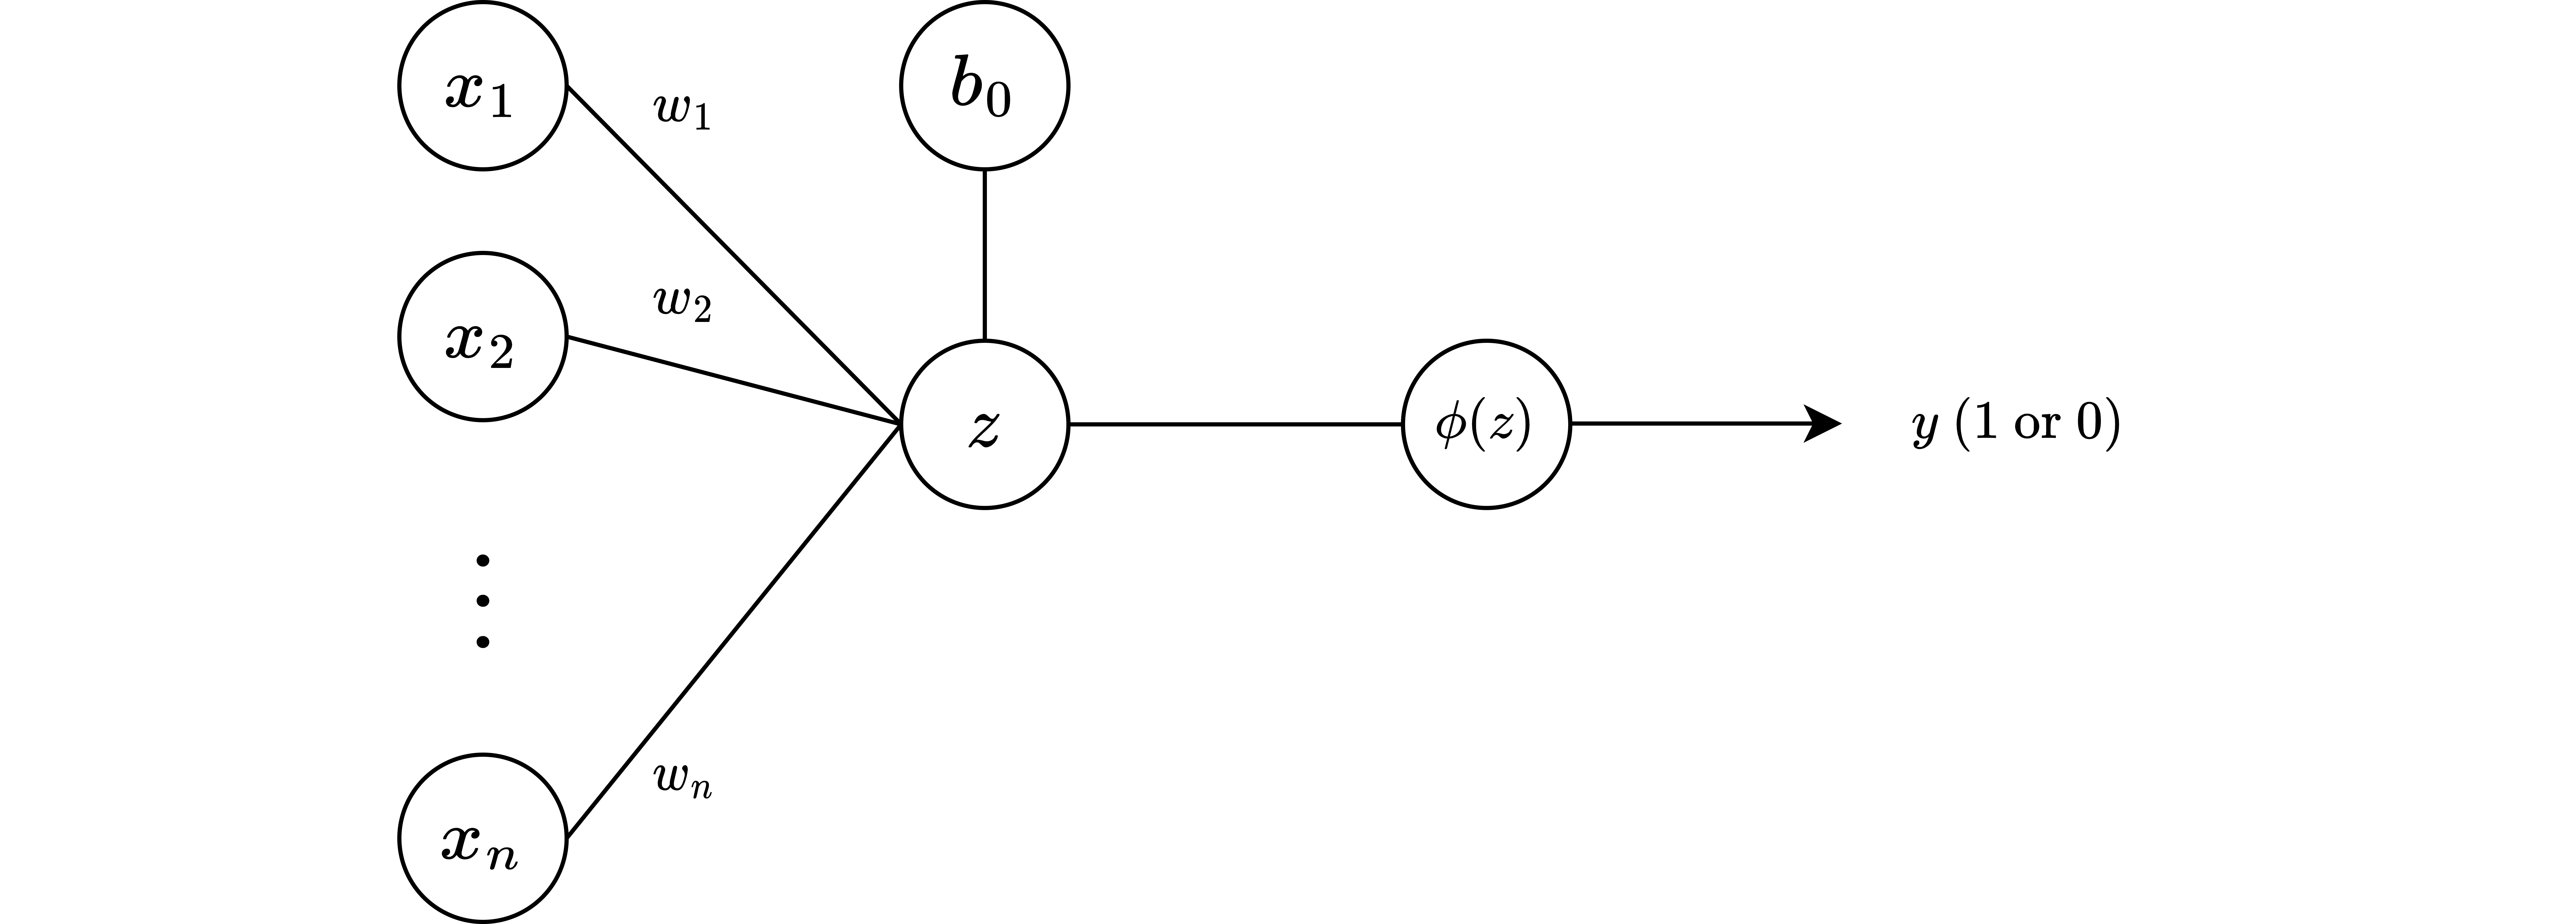
\includegraphics[scale=0.95]{CHAPTER_2/c2_fig_perceptron_2_draw.png}
  \caption{Rosenblatt perceptron}
  \label{rosenblatt_perceptron}
\end{figure}

\noindent Let $\textbf{x}$ be a vector of inputs where each $x_i \in \mathbb{Z}$ and $\textbf{w}$ be a vector of weights corresponding to the input signals where each $w_i \in \mathbb{Z}$. 
\begin{align}
  \begin{matrix}
    \textbf{x} = \begin{bmatrix}
      x_{0}, x_{1}, \dots, x_{n}
    \end{bmatrix}^T&\text{and} & \textbf{w} = \begin{bmatrix}
      w_{0}, w_{1}, \dots, w_{n}
    \end{bmatrix}^T
  \end{matrix} \nonumber
\end{align}
\noindent Then, the mathematical definition of the perceptron is given by
\begin{align}
  \phi(z) = \begin{cases}
    1 & \text{if } \mathbf{w^Tx + b}\geq  0\\
    0 & \text{otherwise}
    \label{eq:mcp_neuron}
  \end{cases}
\end{align}
\vspace{5mm}
\\
where $\phi(z)$ is known as the hard delimiter.
\vspace{5mm}
\\
%\noindent Consider the two sets of point \textbf{A} and \textbf{B}
\noindent Consider sets in $\mathbb{R}^2$ given by $\textbf{A}=\{a_1\}$ and $\textbf{B}=\{b_1,\,b_2\}$ where $a_1=(1,\,2)^T$, $b_1=(-1,\,2)^T$ and $b_2=(0,\,-1)^T$. The two sets are linearly separable in $\mathbb{R}^2$ as shown in Figure~\ref{fig:perceptron_example_2}. There are an infinite number of separating hyperplanes. One separating hyperplane through the origin is the line $x_1+x_2=0$. The normal vector to this line is given by $w=\left(1,\,1\right)$ and this line points in the direction of $A$. 
\begin{align}
  \textbf{A} =
  \begin{Bmatrix}
    \begin{bmatrix}
      1 \\ 
      2
    \end{bmatrix}
  \end{Bmatrix}
   \, \, \, 
  \textbf{B} =
\begin{Bmatrix}
  \begin{bmatrix}
    -1 \\
    2
  \end{bmatrix},
  \begin{bmatrix}
    0 \\
    -1
  \end{bmatrix}
  \end{Bmatrix}
\end{align}
%and fitting the perceptron function (\refeq{eq:mcp_neuron}) to learn how to classify points in each respective set. Let set \textbf{A} and \textbf{B} be class 1 and 0 respectively.
%\begin{figure}[ht]
%  \centering
%  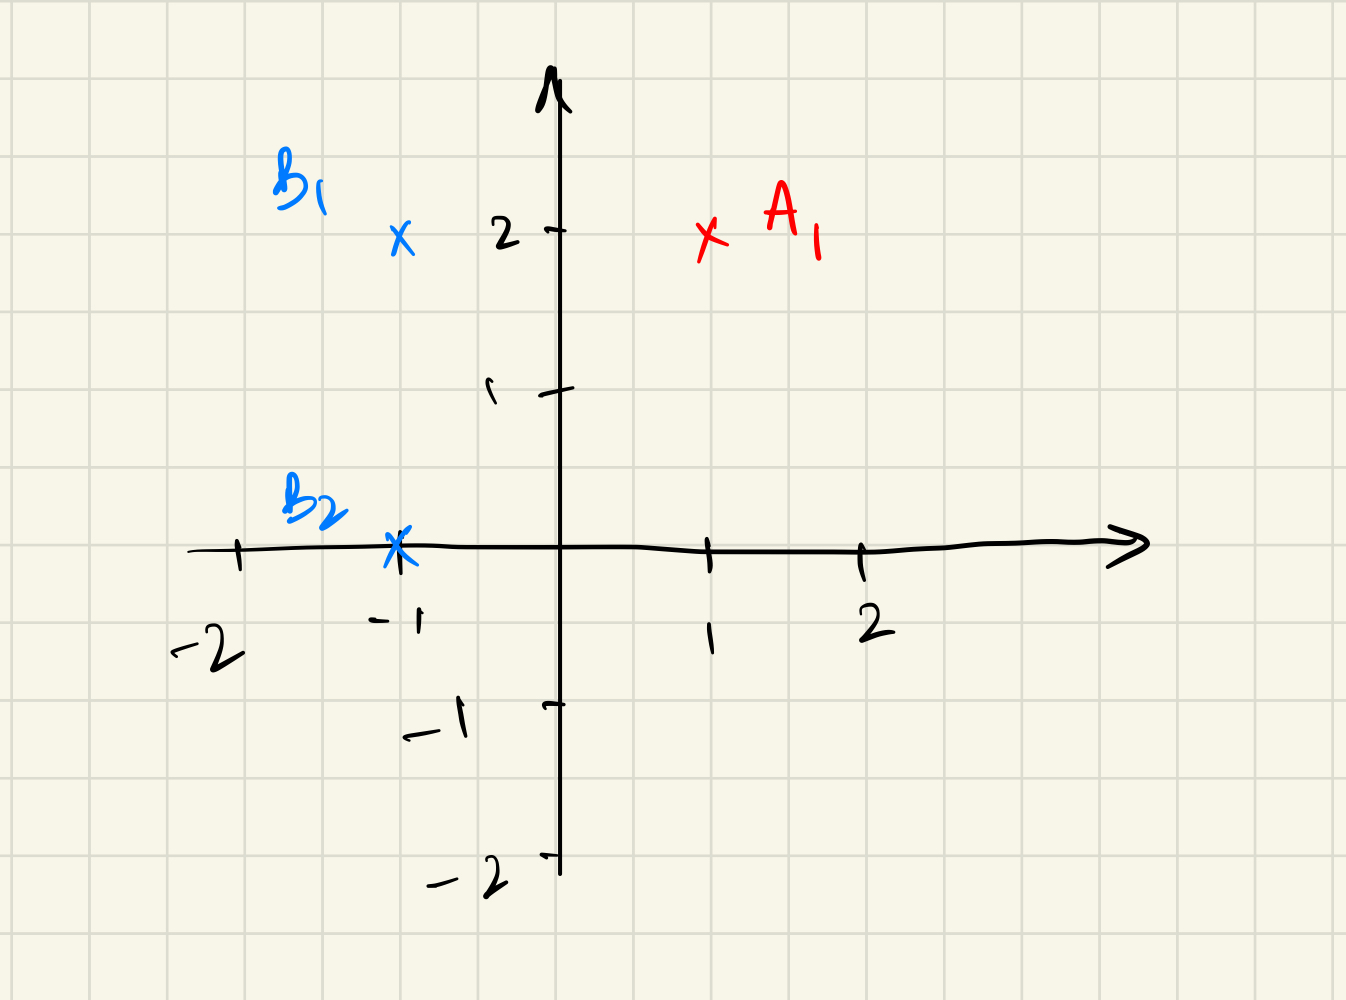
\includegraphics[scale=0.15]{CHAPTER_2/c2_fig_perceptron_example_1.jpeg}
%  \caption{Caption}
%  \label{fig:perceptron_example_1}
%\end{figure}\\
%From \ref{fig:perceptron_example_1}, we can separate the two classes by a single line. Consider the random separating line passing through the origin (this will set the value of $x_0$ in (\refeq{eq:mcp_neuron}) to 0).\\
\begin{figure}[H]
  \centering
  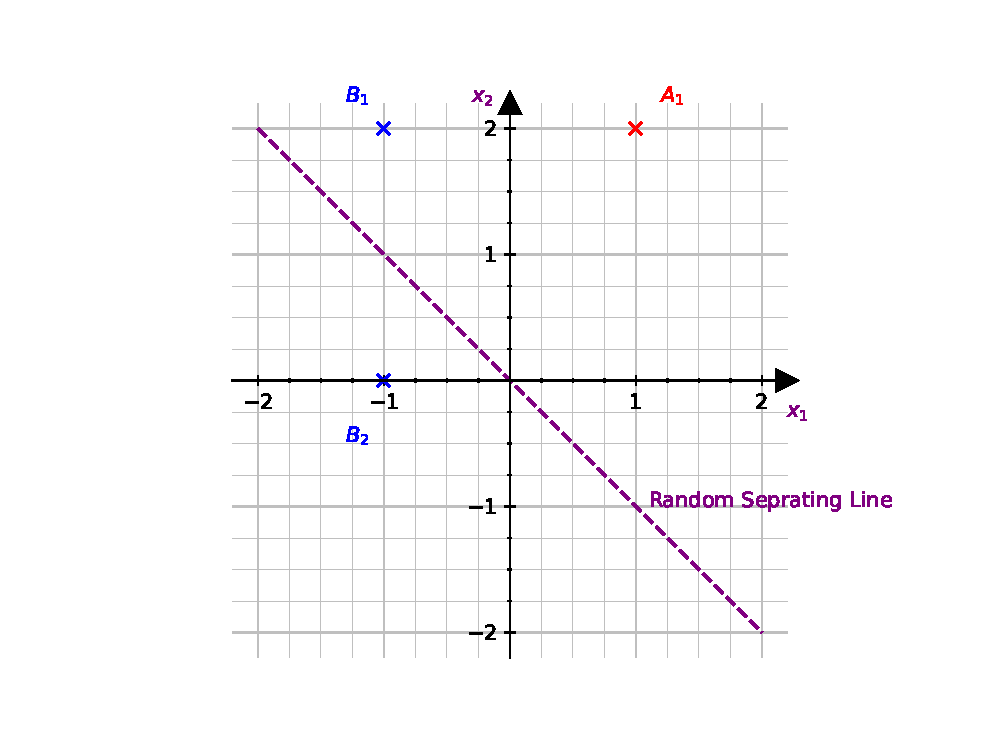
\includegraphics[scale=0.75]{CHAPTER_2/c2_fig_perceptron_example_2_python.eps}
  \caption{Set $\mathbf{A}$ and $\mathbf{B}$ with a random separating line}
  \label{fig:perceptron_example_2}
\end{figure}
%The equation of the random line is given by
%\begin{align}
%  x_1 = - x_2
%\end{align}
\noindent Comparing to the equation (\refeq{eq:mcp_neuron}); we can deduce that 
\begin{align}
  \begin{matrix}
    w_1 = 1 & w_2 = 1
  \end{matrix}
\end{align}
Visually, we can already see that the separating line does not split the points properly. The computation of the binary classification using the random line is given by
\begin{align*}
  \phi(A_1) &= \phi\begin{pmatrix}
    \begin{bmatrix}
      1\\
      1
    \end{bmatrix}.\begin{bmatrix}
      1 \\
      2
    \end{bmatrix}
  \end{pmatrix} = \phi(3) = 1 \\
  \phi(B_1) &= f\begin{pmatrix}
    \begin{bmatrix}
      1\\
      1
    \end{bmatrix}.\begin{bmatrix}
      -1 \\
      2
    \end{bmatrix}
  \end{pmatrix} = \phi(1) = 1 \\
  \phi(B_2) &= f\begin{pmatrix}
    \begin{bmatrix}
      1\\
      1
    \end{bmatrix}.\begin{bmatrix}
      -1 \\
      0
    \end{bmatrix}
  \end{pmatrix} = \phi(-1) = 0
\end{align*}
The computation confirms the visual representation and groups $\textbf{A}_1$ and $\textbf{B}_1$ together and $\textbf{B}_2$ separated which is incorrect. We can either alter the separating line (by moving the weight vector) with respect to $\textbf{A}_1$ and/or $\textbf{B}_1$.
\begin{figure}[H]
  \centering
  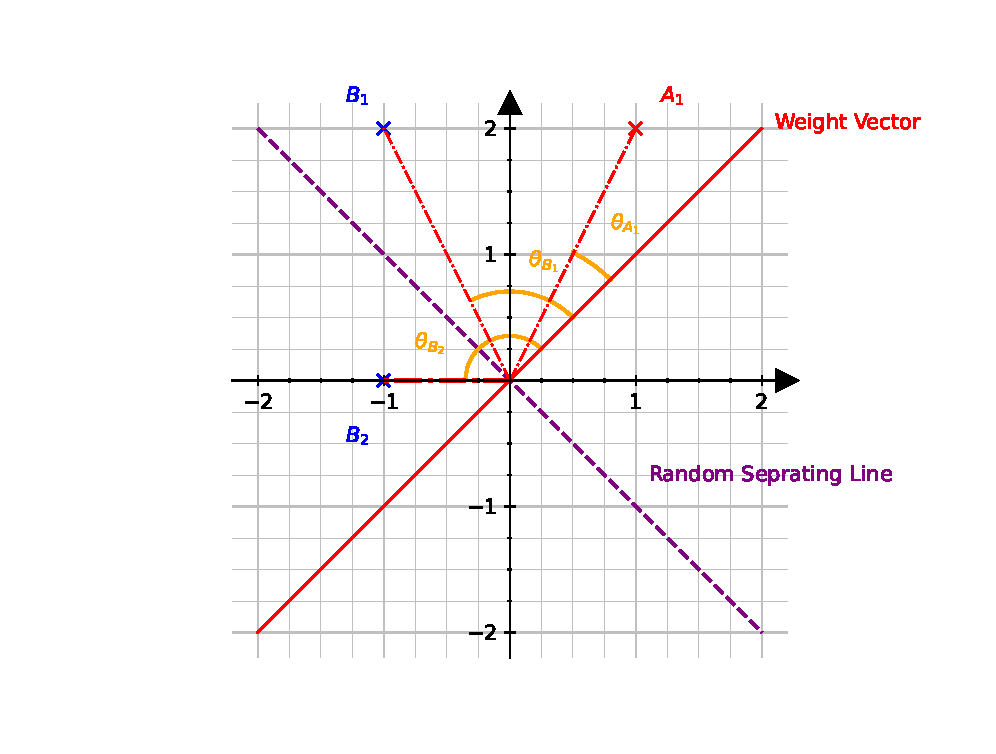
\includegraphics[scale=0.9]{CHAPTER_2/c2_fig_perceptron_example_3_python.eps}
  \caption{Set $\mathbf{A}$ and $\mathbf{B}$ with a random separating line and its weight vector}
  \label{fig:perceptron_example_3}
\end{figure}
\noindent Since $\textbf{B}_1$ is incorrectly classified, using the property of subtraction of vectors; we move the weight vector ($\textbf{w}$) away from $\textbf{B}_1$ and check the classification again.
\begin{align}
  \textbf{w}^{(1)} &= \textbf{w} - \textbf{B}_1 \\
  &= \begin{bmatrix}
    1 \\
    1
  \end{bmatrix} - \begin{bmatrix}
    -1 \\
    2
  \end{bmatrix} \\
  & = \begin{bmatrix}
    2 \\
    -1
  \end{bmatrix}
\end{align}
\begin{figure}[H]
  \centering
  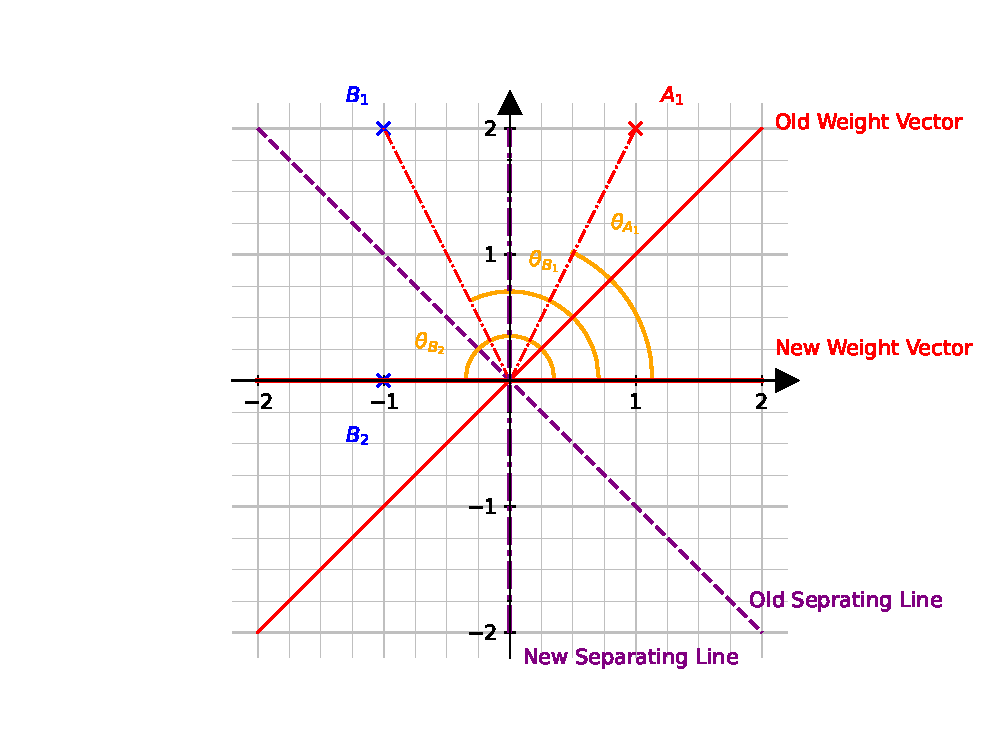
\includegraphics[scale=0.90]{CHAPTER_2/c2_fig_perceptron_example_4_python.eps}
  \caption{Set $\mathbf{A}$ and $\mathbf{B}$ after adjusting the separating line and its weight vector}
  \label{fig:perceptron_example_4}
\end{figure}
\noindent Based on the new separating line, we can observe visually that the points are correctly classified. The computation of the binary classification using the new separating line $\textbf{w}^{(1)}$ is given by
\begin{align*}
  \phi(A_1) &= \phi\begin{pmatrix}
    \begin{bmatrix}
      2\\
      -1
    \end{bmatrix}.\begin{bmatrix}
      1 \\
      2
    \end{bmatrix}
  \end{pmatrix} = \phi(0) = 1 \\
  \phi(B_1) &= \phi\begin{pmatrix}
    \begin{bmatrix}
      2\\
      -1
    \end{bmatrix}.\begin{bmatrix}
      -1 \\
      2
    \end{bmatrix}
  \end{pmatrix} = \phi(-4) = 0 \\
  \phi(B_2) &= \phi\begin{pmatrix}
    \begin{bmatrix}
      2\\
      -1
    \end{bmatrix}.\begin{bmatrix}
      -1 \\
      0
    \end{bmatrix}
  \end{pmatrix} = \phi(-2) = 0
\end{align*}
Thus, the perceptron learned how to classify the two sets of points. The function $f(\textbf{x})$ could be re-used to classify new points added to the sets.
\vspace{15mm}

\noindent\textbf{Perceptron Algorithm}

\noindent The perceptron algorithm adjusts the weights and as a result, the hard delimiter as well in order to linearly separate a set of binary labelled input.

\begin{algorithm}[H]
\caption{Perceptron Algorithm}\label{alg:perceptron_algorithm}
\begin{algorithmic}[1]
\Require \\
Let $t=0$ and $\textbf{w} = \begin{bmatrix}
  0 & 0 & \dots & 0
\end{bmatrix}^T$ \\
Consider the training set D $s.t$ $D = C_1 \cup C_2$  \\
$C_1$ $\leftarrow$ input with label 1 \\
$C_2$ $\leftarrow$ input with label 0\\
\textbf{Start}
\While{!convergence}
  \State Select a random input $\textbf{x}$
  \If{$\textbf{x}\in A$ and $\textbf{w}.\textbf{x}<0$}
  \State $\textbf{w} = \textbf{w} + \textbf{x}$
  \EndIf
  \If{$\textbf{x}\in B$ and $\textbf{w}.\textbf{x}\geq0$}
  \State $\textbf{w} = \textbf{w} - \textbf{x}$
  \EndIf
\EndWhile
\end{algorithmic}
\end{algorithm}
\noindent If the input data are binary and linearly separable; then algorithm (\ref{alg:perceptron_algorithm}) converges. The proof of convergence of the algorithm is known as the \textbf{perceptron convergence theorem}.\\
%\section{Perceptron Convergence Theorem}
\textbf{Theorem}\\
Consider algorithm (\ref{alg:perceptron_algorithm}) and let $D$ be a set of training vectors which are linearly separable. Let $\textbf{w}^{*}$ be the weight vectors which defines the separating line with $||\textbf{w}^{*}|| = 1$. Then the perceptron convergence theorem states that the number of mistakes $m$ made by the perceptron algorithm satisfies 
\begin{align}
  \begin{matrix}
    m \leq \dfrac{1}{\gamma^2} & \text{where} & \gamma = \underset{\textbf{x}\in D}{\min} \dfrac{|{\textbf{w}^*}^T\textbf{x}|}{||\textbf{x}||_2}
  \end{matrix}
\end{align}
\textbf{Note}
\begin{enumerate}
  \item Since, $||\textbf{w}^{*}|| = 1 \implies \cos (\theta) = \dfrac{{\textbf{w}^*}^T\textbf{x}}{||\textbf{x}||_2}$
  \item If $||\textbf{x}||_2 = 1$, that is, we scale all the training examples to have unit norm (which has no effect their orientation), then $\gamma = \underset{\textbf{x}\in D}{\min} |{\textbf{w}^*}^T\textbf{x}|$ is the minimum distance from any example $\textbf{x} \in D$ to the separating line.
\end{enumerate}
\textbf{Proof}\\
We first prove the inequality given by 
\begin{align}
  (\textbf{w}^ {(t+1)})^T\textbf{w}^{*} \geq (\textbf{w}^ {(t)})^T\textbf{w}^{*} + \gamma
  \label{eq:per_cov_ine_1}
\end{align}
\indent \textbf{State 1} \\
In state 1, let us consider \textbf{x} being positive ($\textbf{x} \in C_1$) and incorrectly classified then
\begin{align}
  \nonumber
  (\textbf{w}^ {(t+1)})^T\textbf{w}^{*} = (\textbf{w}^ {(t)} + \textbf{x})^T\textbf{w}^{*} =   (\textbf{w}^ {(t)})^T\textbf{w}^{*} + \textbf{x}^T\textbf{w}^{*}
\end{align}
Assuming that all $||\textbf{x}||_2 = 1$ then $\textbf{x}^T\textbf{w}^{*} \geq \gamma$ since $\gamma$ is the minimum. 
\begin{align}
  \label{eq:per_cov_ine_2}
  (\textbf{w}^ {(t+1)})^T\textbf{w}^{*} \geq (\textbf{w}^ {(t)})^T\textbf{w}^{*} + \gamma
\end{align}
Thus, we have proved (\ref{eq:per_cov_ine_1})  under \textbf{State 1}.\\
\indent \textbf{State 2} \\
In state 2, let us consider \textbf{x} being negative ($\textbf{x} \in C_2$) and incorrectly classified then
\begin{align}
  \nonumber
  (\textbf{w}^ {(t+1)})^T\textbf{w}^{*} = (\textbf{w}^ {(t)} - \textbf{x})^T\textbf{w}^{*} =   (\textbf{w}^ {(t)})^T\textbf{w}^{*} - \textbf{x}^T\textbf{w}^{*}
\end{align}
Since $\textbf{x} \in C_2 \implies |{\textbf{w}^*}^T\textbf{x}| = - \textbf{x}^T\textbf{w}^* \geq 0$ and $|\textbf{x}^T\textbf{w}^{*}| \geq \gamma$
\begin{align}
  \nonumber
  (\textbf{w}^ {(t+1)})^T\textbf{w}^{*} &= (\textbf{w}^ {(t)})^T\textbf{w}^{*} + |{\textbf{w}^*}^T\textbf{x}| \\
  \label{eq:per_cov_ine_3}
  (\textbf{w}^ {(t+1)})^T\textbf{w}^{*} &\geq (\textbf{w}^ {(t)})^T\textbf{w}^{*} + \gamma
\end{align}
Thus, we have proved (\ref{eq:per_cov_ine_1})  under \textbf{State 2}.\\
From (\ref{eq:per_cov_ine_2}) and (\ref{eq:per_cov_ine_3}), we have shown that $\forall \textbf{x}\in D$ that inequality (\ref{eq:per_cov_ine_1}) holds.\\
Assume that the inequality (\ref{eq:per_cov_ine_1}) holds for an arbitrary integer value $m$ and $m-1$
\begin{align}
  \label{eq:induction_1}
  (\textbf{w}^ {(m)})^T\textbf{w}^{*} \geq (\textbf{w}^ {(m-1)})^T\textbf{w}^{*} + \gamma \\
  \label{eq:induction_2}
  (\textbf{w}^ {(m-1)})^T\textbf{w}^{*} \geq (\textbf{w}^ {(m-2)})^T\textbf{w}^{*} + \gamma 
\end{align}
Merging inequality (\ref{eq:induction_1}) and (\ref{eq:induction_2}) gives us
\begin{align}
  \label{eq:induction_3}
  (\textbf{w}^ {(m)})^T\textbf{w}^{*} \geq (\textbf{w}^ {(m-2)})^T\textbf{w}^{*} + 2\gamma
\end{align}
Hence, by induction, after $M$ mistakes, inequality (\ref{eq:induction_3}) becomes
\begin{align}
  \label{eq:induction_starts}
  (\textbf{w}^ {(m)})^T\textbf{w}^{*} \geq (\textbf{w}^ {(0)})^T\textbf{w}^{*} + m\gamma
\end{align}
Since $\textbf{w}^{(0)} = \mathbf{0}$ (the zero vector), we have
\begin{align}
  \label{eq:perp_cov_result1}
  (\textbf{w}^ {(m)})^T\textbf{w}^{*} \geq m\gamma
\end{align}
Next, we show that 
\begin{align}
  ||{\textbf{w}^{(t+1)}}||_{2}^{2} \leq ||{\textbf{w}^{(t)}}||_{2}^{2} + 1
  \label{eq:induction_proof_part2}
\end{align}
\indent \textbf{State 1} \\
Consider the same state 1 as before, thus we have
\begin{align}
  \begin{matrix}
    \label{eq:state1_conditions}
    (\textbf{w}^ {(t)})^T\textbf{x} \leq 0 & \text{and} & \textbf{w}^ {(t+1)} = \textbf{w}^{(t)} + \textbf{x}
  \end{matrix}
\end{align}
then
\begin{align}
  \nonumber
  ||\textbf{w}^{(t+1)}||_{2}^{2} &= ( \textbf{w}^{(t)} + \textbf{x})^T( \textbf{w}^{(t)} + \textbf{x}) \\
  \nonumber
  &=( \textbf{w}^{(t)} + \textbf{x})^T\textbf{w}^{(t)} + ( \textbf{w}^{(t)} + \textbf{x})^T\textbf{x} \\
  \nonumber
  &= (\textbf{w}^{(t)})^T\textbf{w}^{(t)} + \textbf{x}^T\textbf{w}^{(t)} + (\textbf{w}^{(t)})^T\textbf{x} + \textbf{x}^T\textbf{x}\\
  &= (\textbf{w}^{(t)})^T\textbf{w}^{(t)} + 2 (\textbf{w}^{(t)})^T\textbf{x}  + \textbf{x}^T\textbf{x}
  \label{eq:state_1_proof}
\end{align}
Since (\ref{eq:state1_conditions}) and $\textbf{x}^T\textbf{x} = 1$, equation (\ref{eq:state_1_proof}) becomes
\begin{align}
  ||{\textbf{w}^{(t+1)}}||_{2}^{2} \leq ||{\textbf{w}^{(t)}}||_{2}^{2} + 1
\end{align}\\
\indent \textbf{State 2} \\
Consider the same state 2 as before, thus we have
\begin{align}
  \begin{matrix}
    \label{eq:state2_conditions}
    (\textbf{w}^ {(t)})^T\textbf{x} > 0 & \text{and} & \textbf{w}^ {(t+1)} = \textbf{w}^{(t)} - \textbf{x}
  \end{matrix}
\end{align}
then
\begin{align}
  \nonumber
  ||\textbf{w}^{(t+1)}||_{2}^{2} &= ( \textbf{w}^{(t)} - \textbf{x})^T( \textbf{w}^{(t)} - \textbf{x}) \\
  \nonumber
  &=( \textbf{w}^{(t)} - \textbf{x})^T\textbf{w}^{(t)} - ( \textbf{w}^{(t)} - \textbf{x})^T\textbf{x} \\
  \nonumber
  &= (\textbf{w}^{(t)})^T\textbf{w}^{(t)} - \textbf{x}^T\textbf{w}^{(t)} - (\textbf{w}^{(t)})^T\textbf{x} + \textbf{x}^T\textbf{x}\\
  &= (\textbf{w}^{(t)})^T\textbf{w}^{(t)} - 2 (\textbf{w}^{(t)})^T\textbf{x}  + \textbf{x}^T\textbf{x}
  \label{eq:state_2_proof}
\end{align}
Since (\ref{eq:state2_conditions}) and $\textbf{x}^T\textbf{x} = 1$, equation (\ref{eq:state_2_proof}) becomes
\begin{align}
  ||{\textbf{w}^{(t+1)}}||_{2}^{2} \leq ||{\textbf{w}^{(t)}}||_{2}^{2} + 1
\end{align}
Thus, we have proved (\ref{eq:induction_proof_part2}) under \textbf{State 2}.\\
By the same induction defined in (\ref{eq:induction_starts}), we have
\begin{align}
  \label{eq:perp_cov_result2}
  ||\textbf{w}^{(m)}||_{2}^{2} \leq m
\end{align}
Finally, we merge result (\ref{eq:perp_cov_result1}) and (\ref{eq:perp_cov_result2}) using the Cauchy-Schwarz (CS) inequality \\
Recall that the CS inequality is given by
\begin{align}
  \label{eq:CS_inquality}
  |{\textbf{w}^*}^T\textbf{x}| \leq ||\textbf{w}^{*}||_2 ||\textbf{x}||_2
\end{align}
Hence, using (\ref{eq:CS_inquality}) we get
\begin{align}
  \label{eq:after_cs}
  |(\textbf{w}^{m})^T\textbf{w}^{*}| \leq ||(\textbf{w}^{m})^T||_2  ||\textbf{w}^{*}||_2
\end{align}
From the result (\ref{eq:perp_cov_result1}), (\ref{eq:after_cs}) becomes
\begin{align}
  m\gamma \leq |(\textbf{w}^{m})^T\textbf{w}^{*}| \leq ||(\textbf{w}^{m})^T||_2  ||\textbf{w}^{*}||_2
\end{align}
Using the result (\ref{eq:perp_cov_result2}) and the fact that $||\textbf{w}^{*}||_{2} = 1$, we get
\begin{align}
  \nonumber
  m\gamma &\leq ||(\textbf{w}^{m})^T||_2 \\
  m^2 {\gamma}^2 &\leq ||(\textbf{w}^{m})^T||_{2}^{2} \\
  m^2 {\gamma}^2 &\leq m \\
  m &\leq \dfrac{1}{\gamma^2}
\end{align}
This proves the Perceptron Convergence Theorem that the number of mistakes is at most $\dfrac{1}{\gamma^2}$, where $\gamma$ is the margin.\vspace*{5mm}\\
%\section{Solving Gate Problems}
Even though the perceptron converges, alone it is not always a good model to solve binary classification problem. It has certain limitation by nature of its definition. Consider the logic functions AND, OR and XOR across these 4 points:
\begin{align}
  \begin{matrix}
    \textbf{p}_1 = \begin{bmatrix}
      0 \\
      0
    \end{bmatrix},
    \textbf{p}_2 = \begin{bmatrix}
      1 \\
      0
    \end{bmatrix},
    \textbf{p}_3 = \begin{bmatrix}
      1 \\
      1
    \end{bmatrix},
    \textbf{p}_4 = \begin{bmatrix}
      0 \\
      1
    \end{bmatrix}  
  \end{matrix}
\end{align}
\subsubsection*{AND Function}
The AND function returns a value of 1 if both of the inputs is 1. Let $f$ be the AND function such that
\begin{align}
\begin{matrix}
  \nonumber
  f(\textbf{p}_1) = 0 & f(\textbf{p}_2) = 0 & f(\textbf{p}_3) = 1 & f(\textbf{p}_4) = 0
\end{matrix}  
\end{align}
Consider the AND function with the separating line below
\begin{figure}[ht]
  \centering
  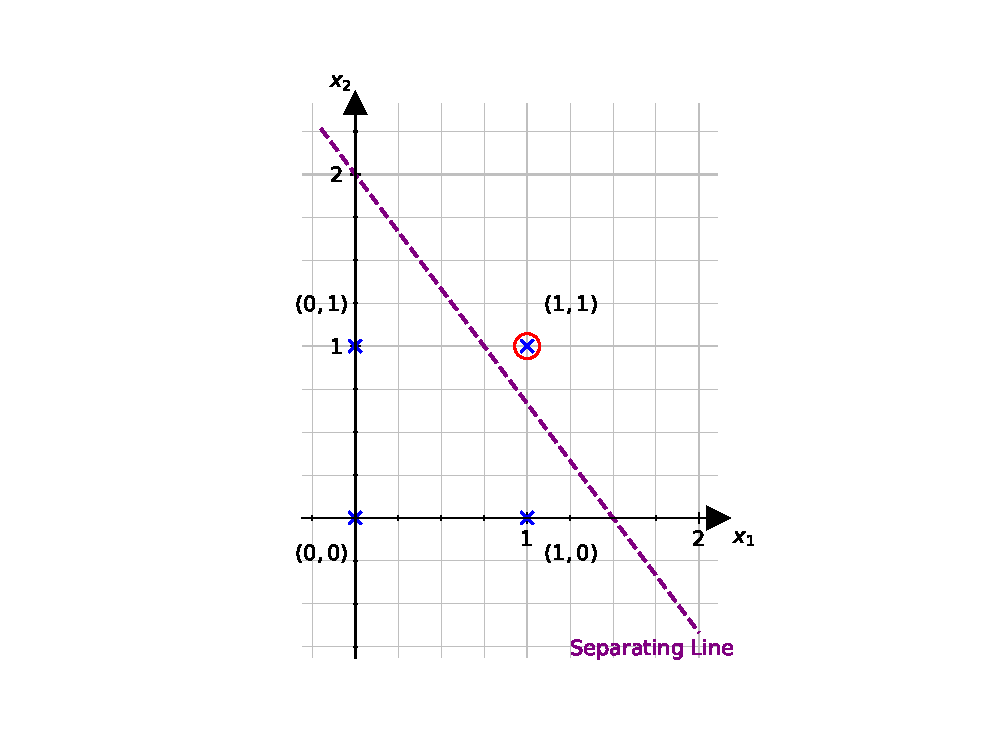
\includegraphics[scale=0.75]{CHAPTER_2/c2_fig_AND_function_python.eps}
  \caption{AND Function with separating line}
  \label{AND_function_2}
\end{figure}\\
The equation of the separating line in figure \ref{AND_function_2} is given by
\begin{align}
  x_1 + x_2 -1.5 = 0
\end{align}
We can transform the separating line in the form of $\textbf{w}^T\textbf{x} = 0$ to fit the perceptron.\\
Let 
\begin{align}
  \begin{matrix}
    \textbf{w} = \begin{bmatrix}
      -1.5 \\
      1 \\
      1
    \end{bmatrix} & \text{and} & \textbf{x} = \begin{bmatrix}
      1 \\
      x_1 \\
      x_2
    \end{bmatrix}
  \end{matrix}
\end{align}
Applying function (\ref{eq:mcp_neuron}) on each point to check whether they are correctly classified.
\begin{align}
  \nonumber
  \begin{matrix}
    \phi(p_1) = \phi\begin{pmatrix}
      \begin{bmatrix}
        -1.5 \\
        1 \\
        1 
      \end{bmatrix}.\begin{bmatrix}
        1 \\
        0 \\
        0
      \end{bmatrix}
    \end{pmatrix} = \phi(-1.5) = 0 
  \end{matrix}
\end{align}
\begin{align}
  \nonumber
  \begin{matrix}
    \phi(p_2) = \phi\begin{pmatrix}
      \begin{bmatrix}
        -1.5 \\
        1 \\
        1 
      \end{bmatrix}.\begin{bmatrix}
        1 \\
        1 \\
        0
      \end{bmatrix}
    \end{pmatrix} = \phi(-0.5) = 0
  \end{matrix}
\end{align}
\begin{align}
  \nonumber
  \begin{matrix}
    \phi(p_3) = \phi\begin{pmatrix}
      \begin{bmatrix}
        -1.5 \\
        1 \\
        1 
      \end{bmatrix}.\begin{bmatrix}
        1 \\
        1 \\
        1
      \end{bmatrix}
    \end{pmatrix} = \phi(0.5) = 1
  \end{matrix}
\end{align}
\begin{align}
  \nonumber
  \begin{matrix}
    \phi(p_4) = \phi\begin{pmatrix}
      \begin{bmatrix}
        -1.5 \\
        1 \\
        1 
      \end{bmatrix}.\begin{bmatrix}
        1 \\
        0 \\
        1
      \end{bmatrix}
    \end{pmatrix} = \phi(-0.5) = 0
  \end{matrix}
\end{align}
Thus, the perceptron is able to solve the AND function.
\subsubsection*{OR Function}
The OR function returns a value of 1 if either of the inputs is 1. Let $f$ be the OR function such that
\begin{align}
\begin{matrix}
  \nonumber
  f(\textbf{p}_1) = 0 & f(\textbf{p}_2) = 1 & f(\textbf{p}_3) = 1 & f(\textbf{p}_4) = 1
\end{matrix}  
\end{align}
Consider the OR function with the separating line below
\begin{figure}[ht]
  \centering
  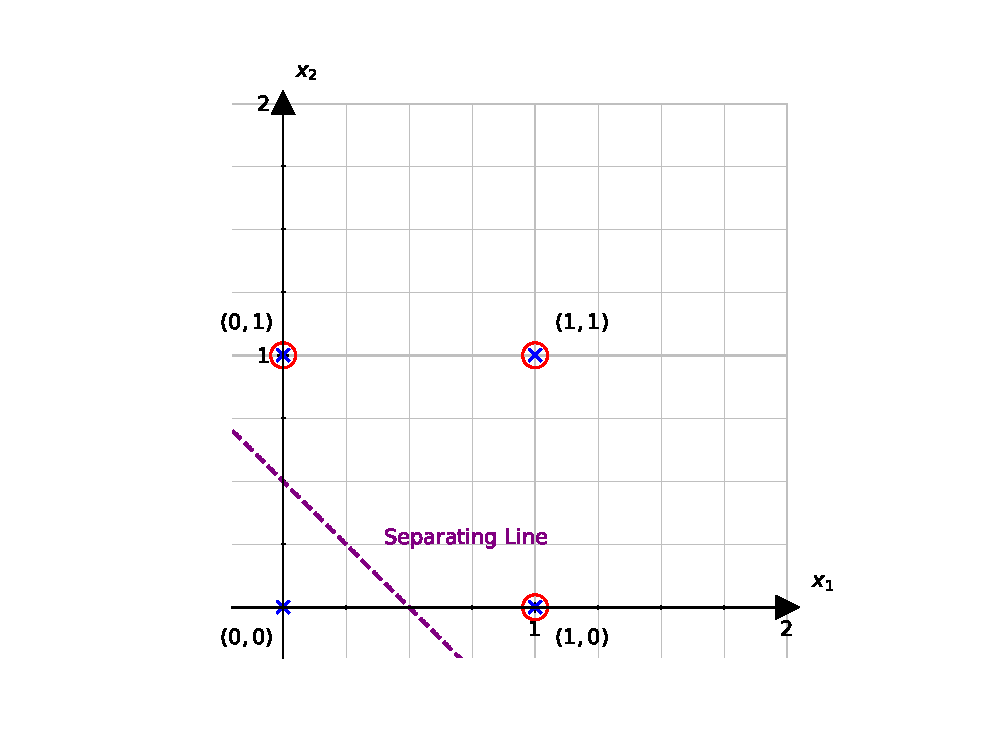
\includegraphics[scale=0.75]{CHAPTER_2/c2_fig_OR_function_python.eps}
  \caption{OR Function with separating line}
  \label{OR_function}
\end{figure}\\
The equation of the separating line in figure \ref{OR_function} is given by
\begin{align}
  x_1 + x_2 - 0.5 = 0
\end{align}
We can transform the separating line in the form of $\textbf{w}^T\textbf{x} = 0$ to fit the perceptron.\\
Let 
\begin{align}
  \begin{matrix}
    \textbf{w} = \begin{bmatrix}
      -0.5 \\
      1 \\
      1
    \end{bmatrix} & \text{and} & \textbf{x} = \begin{bmatrix}
      1 \\
      x_1 \\
      x_2
    \end{bmatrix}
  \end{matrix}
\end{align}
Applying function (\ref{eq:mcp_neuron}) on each point to check whether they are correctly classified.
\begin{align}
  \nonumber
  \begin{matrix}
    \phi(p_1) = \phi\begin{pmatrix}
      \begin{bmatrix}
        -0.5 \\
        1 \\
        1 
      \end{bmatrix}.\begin{bmatrix}
        1 \\
        0 \\
        0
      \end{bmatrix}
    \end{pmatrix} = \phi(-0.5) = 0 
  \end{matrix}
\end{align}
\begin{align}
  \nonumber
  \begin{matrix}
    \phi(p_2) = \phi\begin{pmatrix}
      \begin{bmatrix}
        -0.5 \\
        1 \\
        1 
      \end{bmatrix}.\begin{bmatrix}
        1 \\
        1 \\
        0
      \end{bmatrix}
    \end{pmatrix} = \phi(0.5) = 1
  \end{matrix}
\end{align}
\begin{align}
  \nonumber
  \begin{matrix}
    \phi(p_3) = \phi\begin{pmatrix}
      \begin{bmatrix}
        -0.5 \\
        1 \\
        1 
      \end{bmatrix}.\begin{bmatrix}
        1 \\
        1 \\
        1
      \end{bmatrix}
    \end{pmatrix} = \phi(1.5) = 1
  \end{matrix}
\end{align}
\begin{align}
  \nonumber
  \begin{matrix}
    \phi(p_4) = \phi\begin{pmatrix}
      \begin{bmatrix}
        -0.5 \\
        1 \\
        1 
      \end{bmatrix}.\begin{bmatrix}
        1 \\
        0 \\
        1
      \end{bmatrix}
    \end{pmatrix} = \phi(0.5) = 1
  \end{matrix}
\end{align}
Thus, the perceptron is able to solve the OR function.
\subsubsection*{XOR Function}
The XOR function returns a value of 1 if either of the inputs is 1 but not both. Let $f$ be the XOR function such that
\begin{align}
  \begin{matrix}
    f(\textbf{p}_1)=0,&   f(\textbf{p}_2)=1 ,& f(\textbf{p}_3)=0,&   f(\textbf{p}_4)=1
    \label{eq:XOR_function}    
  \end{matrix}
\end{align}
Consider a plot of the XOR function below 
\begin{figure}[ht]
  \centering
  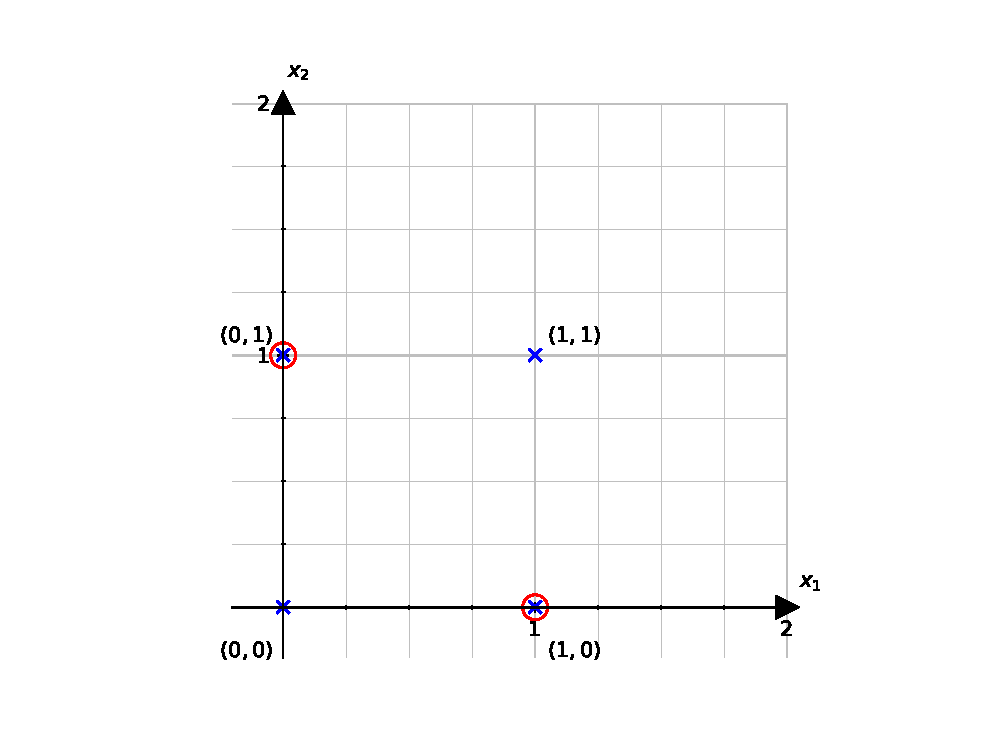
\includegraphics[scale=0.75]{CHAPTER_2/c2_rig_XOR_python.eps}
  \caption{XOR function}
  \label{XOR_function}
\end{figure}\\
From figure \ref{XOR_function}; we can observe that no separating line alone could group the two different classes together. We attempt to find a combination of weight for the perceptron which reduces the error (margin) as much as possible. Let $f^{*}$ be the exact function and $f(\textbf{x},\textbf{w}) = \textbf{w}^T\textbf{x} + b$, where $\textbf{w} = [w_1 \, \, w_2]^T$, be the approximate function. Consider the error function (the difference between the exact and approximate value)
\begin{align}
  \label{eq:error_XOR_prob}
  \mathbb{E}(\textbf{w},b) = \dfrac{1}{4} \sum_{x\in D}(f^{*}(\textbf{x})- \textbf{w}^T\textbf{x}-b)^2
\end{align}
we minimise the error function $\mathbb{E}$ by setting the partial derivatives to 0. The partial derivative with respect to the bias is given by
\begin{align}
  \nonumber
  \dfrac{\partial \mathbb{E}}{\partial b} &= -\dfrac{1}{2} \sum_{x\in D}(f^{*}(\textbf{x})- \textbf{w}^T\textbf{x}-b)\\
  \label{eq:bias_derivative}
  \dfrac{\partial \mathbb{E}}{\partial b} = 0\rightarrow \sum_{x\in D}f^{*}(\textbf{x}) &= \sum_{x\in D}\textbf{w}^T\textbf{x}- \sum_{x\in D}b
\end{align}
The partial derivative with respect to the weight vector is given by
\begin{align}
  \nonumber
  \dfrac{\partial \mathbb{E}}{\partial \textbf{x}} &= \dfrac{1}{2} \sum_{x\in D}(f^{*}(\textbf{x})- \textbf{w}^T\textbf{x}-b) \dfrac{\partial (-\textbf{w}^T\textbf{x})}{\partial \textbf{w}}\\
  \nonumber
  &=-\dfrac{1}{2} \sum_{x\in D}(f^{*}(\textbf{x})- \textbf{w}^T\textbf{x}-b)\textbf{x}\\
  \label{eq:weight_derivative}
  \dfrac{\partial \mathbb{E}}{\partial \textbf{w}} = 0\rightarrow \sum_{x\in D}\textbf{x}f^{*}(\textbf{x}) &= \sum_{x\in D}(\textbf{w}^T\textbf{x})\textbf{x} + b\sum_{x\in D}\textbf{x}
\end{align}
Substituting for values in equation (\ref{eq:bias_derivative})
\begin{align}
  \sum_{x\in D}f^{*}(\textbf{x}) &= f^{*}(\textbf{p}_1) + f^{*}(\textbf{p}_2) + f^{*}(\textbf{p}_3) + f^{*}(\textbf{p}_4) \nonumber \\
  &= 0+1+1+0 \nonumber \\
  & = 2 \\
  \sum_{x\in D}\textbf{w}^T\textbf{x} &= \textbf{w}^T\begin{bmatrix}
    0 \\
    0
  \end{bmatrix} + \textbf{w}^T\begin{bmatrix}
    1 \\
    0
  \end{bmatrix} + \textbf{w}^T\begin{bmatrix}
    1 \\
    1
  \end{bmatrix}+ \textbf{w}^T\begin{bmatrix}
    0 \\
    1
  \end{bmatrix} \nonumber \\
  &= 2w_1 + 2w_2 \\
  \nonumber
  \sum_{x\in D}b &= b \sum_{x\in D} 1 \\&= 4b
\end{align}
Thus, we get
\begin{align}
\nonumber 2 &= 2w_1 + 2w_2 + 4b \\
w_1 + w_2 + 2b &= 1
\label{eq:first_set_normal_eq}
\end{align}
Substituting for values in equation (\ref{eq:weight_derivative})
\begin{align}
  \sum_{x\in D}\textbf{x}f^{*}(\textbf{x}) &= \begin{bmatrix}
    0 \\
    0
  \end{bmatrix}(0) + \begin{bmatrix}
    1 \\
    0
  \end{bmatrix}(1) + \begin{bmatrix}
    1 \\
    1
  \end{bmatrix}(0)+ \begin{bmatrix}
    0 \\
    1
  \end{bmatrix}(1) \nonumber \\
  &= \begin{bmatrix}
    1 \\
    1
  \end{bmatrix}\\
  \nonumber
  \sum_{x\in D}(\textbf{w}^T\textbf{x})\textbf{x} &= \begin{bmatrix}
    w_1 & w_2
  \end{bmatrix} \begin{bmatrix}
    0 \\
    0
  \end{bmatrix} \begin{bmatrix}
    0 \\
    0
  \end{bmatrix} + \begin{bmatrix}
    w_1 & w_2
  \end{bmatrix} \begin{bmatrix}
    1 \\
    0
  \end{bmatrix} \begin{bmatrix}
    1 \\
    0
  \end{bmatrix} \\ \nonumber
  &+ \begin{bmatrix}
    w_1 & w_2
  \end{bmatrix} \begin{bmatrix}
    1 \\
    1
  \end{bmatrix} \begin{bmatrix}
    1 \\
    1
  \end{bmatrix} + \begin{bmatrix}
    w_1 & w_2
  \end{bmatrix} \begin{bmatrix}
    0 \\
    1
  \end{bmatrix} \begin{bmatrix}
    0 \\
    1
  \end{bmatrix} \\
  &= \begin{bmatrix}
    2w_1 + w_2 \\
    w_1 + 2w_2
  \end{bmatrix} \\
  \nonumber
\end{align}
\begin{align}
  b\sum_{x\in D}\textbf{x} &= 
    b\begin{bmatrix}
      0 \\
      0
    \end{bmatrix} + b\begin{bmatrix}
      1 \\
      0
    \end{bmatrix} + b\begin{bmatrix}
      1 \\
      1
    \end{bmatrix} + b\begin{bmatrix}
      0 \\
      1
    \end{bmatrix}\\
  &= b\begin{bmatrix}
    2 \\
    2
  \end{bmatrix}
\end{align}
Thus, we get
\begin{align}
  \label{eq:second_set_normal_eq}
\begin{bmatrix}
  1 \\
  1
\end{bmatrix}  &= \begin{bmatrix}
  2w_1 + w_2 \\
  w_1 + 2w_2
\end{bmatrix} + b\begin{bmatrix}
  2 \\
  2
\end{bmatrix}
\end{align}
From equations (\ref{eq:first_set_normal_eq}) and (\ref{eq:second_set_normal_eq}), we get the set of equations that forms the approximate function with the minimum error
\begin{align}
  w_1 + w_2 + 2b &= 1 \nonumber \\
  2w_1 + w_2 + 2b &= 1 \nonumber\\
  w_1 + 2w_2 + 2b &= 1 \nonumber
\end{align}
Solving the system of linear equations we get
\begin{align}
\begin{matrix}
  w_1 = 0 & w_2 = 0 & b = \dfrac{1}{2}
\end{matrix}  
\end{align}
Hence, the approximate function $f(\textbf{x},\textbf{w})$ is given by
\begin{align}
  f(\textbf{x},\textbf{w}) = \dfrac{1}{2}
\end{align}
\begin{figure}[H]
  \centering
  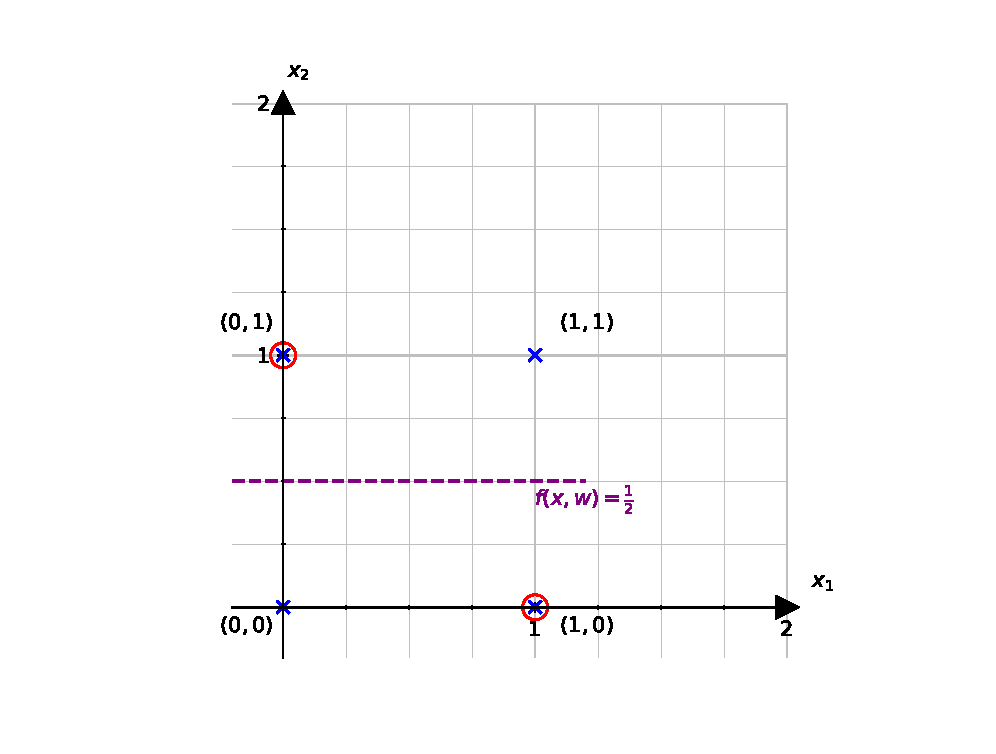
\includegraphics[scale=0.75]{CHAPTER_2/c2_fig_XOR_soln_python.eps}
  \caption{XOR approximate solution}
  \label{fig: approximate_XOR_solution}
\end{figure}
\noindent  Clearly from figure \ref{fig: approximate_XOR_solution}, the perceptron model cannot solve the XOR logic function. The XOR problem is actually not linearly separable. Thus, we introduce \textbf{feedforward networks} to overcome this problem.
\section{Feedforward Network}
We have seen that the single perceptron cannot solve the XOR problem. In order to solve the problem, we use a set of perceptrons that learns two different functions within a connected network.\vspace{5mm} \\
First, let's consider two NOT boolean function $f_1^{*} = x_1 \text{ AND } (\text{NOT }x_2)$ and $f_2^{*} = (\text{NOT }x_1) \text{ AND } x_2$. \vspace{5mm}\\
Consider $f_1^{*}$ which returns 1 if $x_1$ and (not $x_2$) are equal to 1.
\begin{table}[H]
  \begin{center}
    \begin{tabular}{ c c c c}
      $x_1$ & $x_2$ & NOT ($x_2$) & $x_1$ AND (NOT $x_2$) \\
     \hline 
      0 & 0 & 1 & 0 \\  
      1 & 0 & 1 & 1 \\  
      1 & 1 & 0 & 0 \\  
      0 & 1 & 0 & 0 
    \end{tabular}
    \caption{Truth Table for $f_1^{*}$}
  \label{table:truth_table_f_1}
  \end{center}  
\end{table} \vspace{5mm}
\noindent The function $f_1^{*}$ can be separated using the perceptron.
\begin{figure}[H]
  \centering
  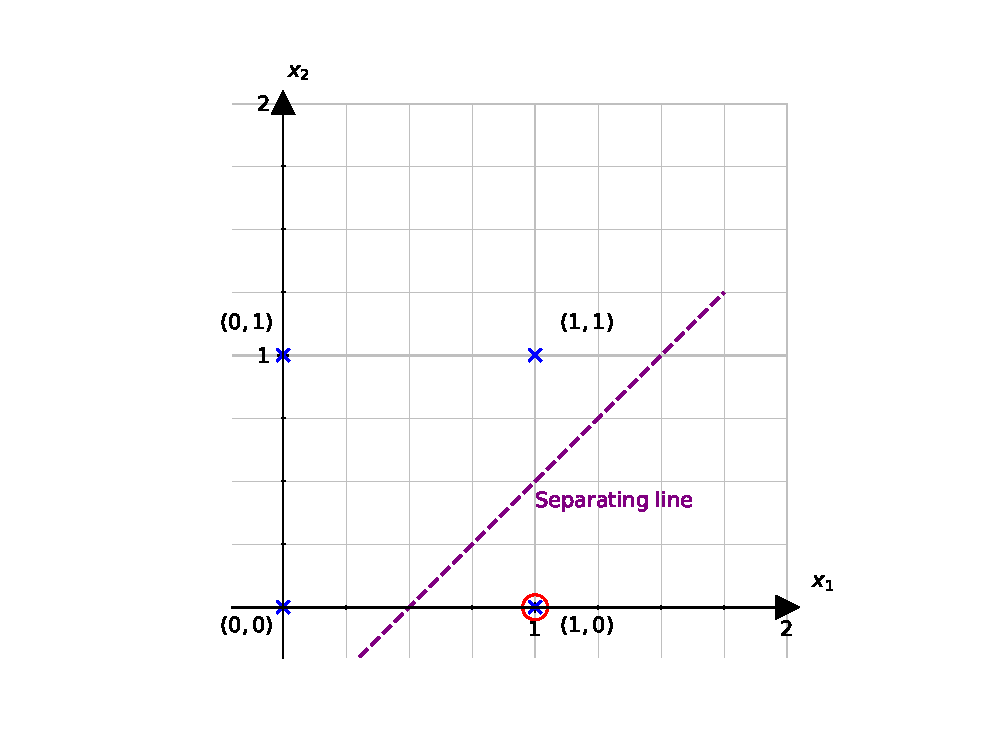
\includegraphics[scale=0.75]{CHAPTER_2/c2_fig_f_1_XOR_python.eps}
  \caption{Representation of Truth Table for function $f_1^{*}$}
  \label{fig:f1_XOR}
\end{figure}
\noindent The equation of the separating line in figure \ref{fig:f1_XOR} is given by
\begin{align}
  x_1 - x_2 - \dfrac{1}{2} = 0
\end{align}
We can transform the separating line in the form of $\textbf{w}^T\textbf{x} = 0$ to fit the perceptron.
\begin{align}
  \label{eq: weight_f_1}
  \begin{matrix}
    \textbf{w} = \begin{bmatrix}
      -0.5 \\
      1 \\
      -1
    \end{bmatrix} & \text{and} & \textbf{x} = \begin{bmatrix}
      1 \\
      x_1 \\
      x_2
    \end{bmatrix}
  \end{matrix}
\end{align}
Similarly, consider $f_2^{*}$ which returns 1 if (not $x_1$) and $x_2$ are equal to 1.
\begin{table}[H]
  \begin{center}
    \begin{tabular}{ c c c c}
      $x_1$ & $x_2$ & NOT ($x_1$) & (NOT $x_1$) AND $x_2$ \\
     \hline 
      0 & 0 & 1 & 0 \\  
      1 & 0 & 0 & 0 \\  
      1 & 1 & 0 & 0 \\  
      0 & 1 & 1 & 1 
    \end{tabular}
    \caption{Truth Table for $f_2^{*}$}
  \label{table:truth_table_f_2}
  \end{center}  
\end{table}
\noindent The function $f_2^{*}$ can be separated using the perceptron.
\begin{figure}[H]
  \centering
  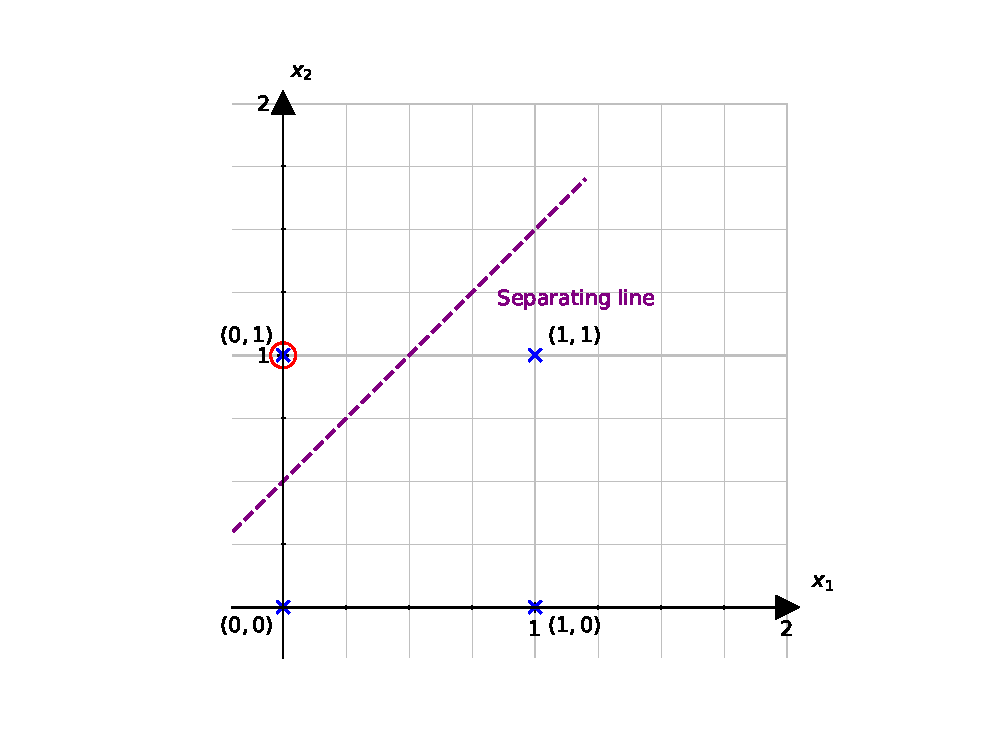
\includegraphics[scale=0.75]{CHAPTER_2/c2_fig_f_2_XOR_python.eps}
  \caption{Representation of Truth Table for function $f_2^{*}$}
  \label{fig:f2_XOR}
\end{figure}
\noindent The equation of the separating line in figure \ref{fig:f2_XOR} is given by
\begin{align}
  -x_1 + x_2 - \dfrac{1}{2} = 0
\end{align}
We can transform the separating line in the form of $\textbf{w}^T\textbf{x} = 0$ to fit the perceptron.
\begin{align}
  \label{eq: weight_f_2}
  \begin{matrix}
    \textbf{w} = \begin{bmatrix}
      -0.5 \\
      -1 \\
      1
    \end{bmatrix} & \text{and} & \textbf{x} = \begin{bmatrix}
      1 \\
      x_1 \\
      x_2
    \end{bmatrix}
  \end{matrix}
\end{align}
Consequently, the XOR function defined in (\ref{eq:XOR_function}) can be expressed as $f^*$ such that
\begin{align}
  \nonumber
  f^*(x_1,x_2) = f_1^*(x_1,x_2) \text{ OR } f_2^*(x_1,x_2)
\end{align}
\begin{table}[H]
  \begin{center}
    \begin{tabular}{ c c c c c}
      $x_1$ & $x_2$ & $f_1^*(x_1,x_2)$ & $f_2^*(x_1,x_2)$ &$f_2^*(x_1,x_2)$ \\
     \hline 
      0 & 0 & 0 & 0 & 0\\  
      1 & 0 & 1 & 0 & 1\\  
      1 & 1 & 0 & 0 & 0\\  
      0 & 1 & 0 & 1 & 1
    \end{tabular}
    \caption{Truth Table for $f^{*}$}
  \label{table:truth_table_f*}
  \end{center}  
\end{table}
\noindent Consider a feedforward network with a hidden layer with two units $h_1$ and $h_2$ such that $h_1$ learns $f_1^*(x_1,x_2)$ and $h_2$ learns $f_2^*(x_1,x_2)$.
\begin{align}
  h_1 &= f_1^*(x_1,x_2) \nonumber\\
  &= \phi(z_1) \nonumber
\end{align}
where $z_1 = w_{11}x_1 + w_{12}x_2 + b_1$ and $w_{11} = 1$, $w_{12} = -1$ and $b_1=-0.5$ from separating line in (\ref{eq: weight_f_1}).
\begin{align}
  h_2 &= f_2^*(x_1,x_2) \nonumber\\
  &= \phi(z_2) \nonumber
\end{align}
where $z_2 = w_{21}x_1 + w_{22}x_2 + b_1$ and $w_{21} = -1$, $w_{22} = 1$ and $b_2 = -0.5$ from separating line in (\ref{eq: weight_f_2}).
\begin{figure}[ht]
  \centering
  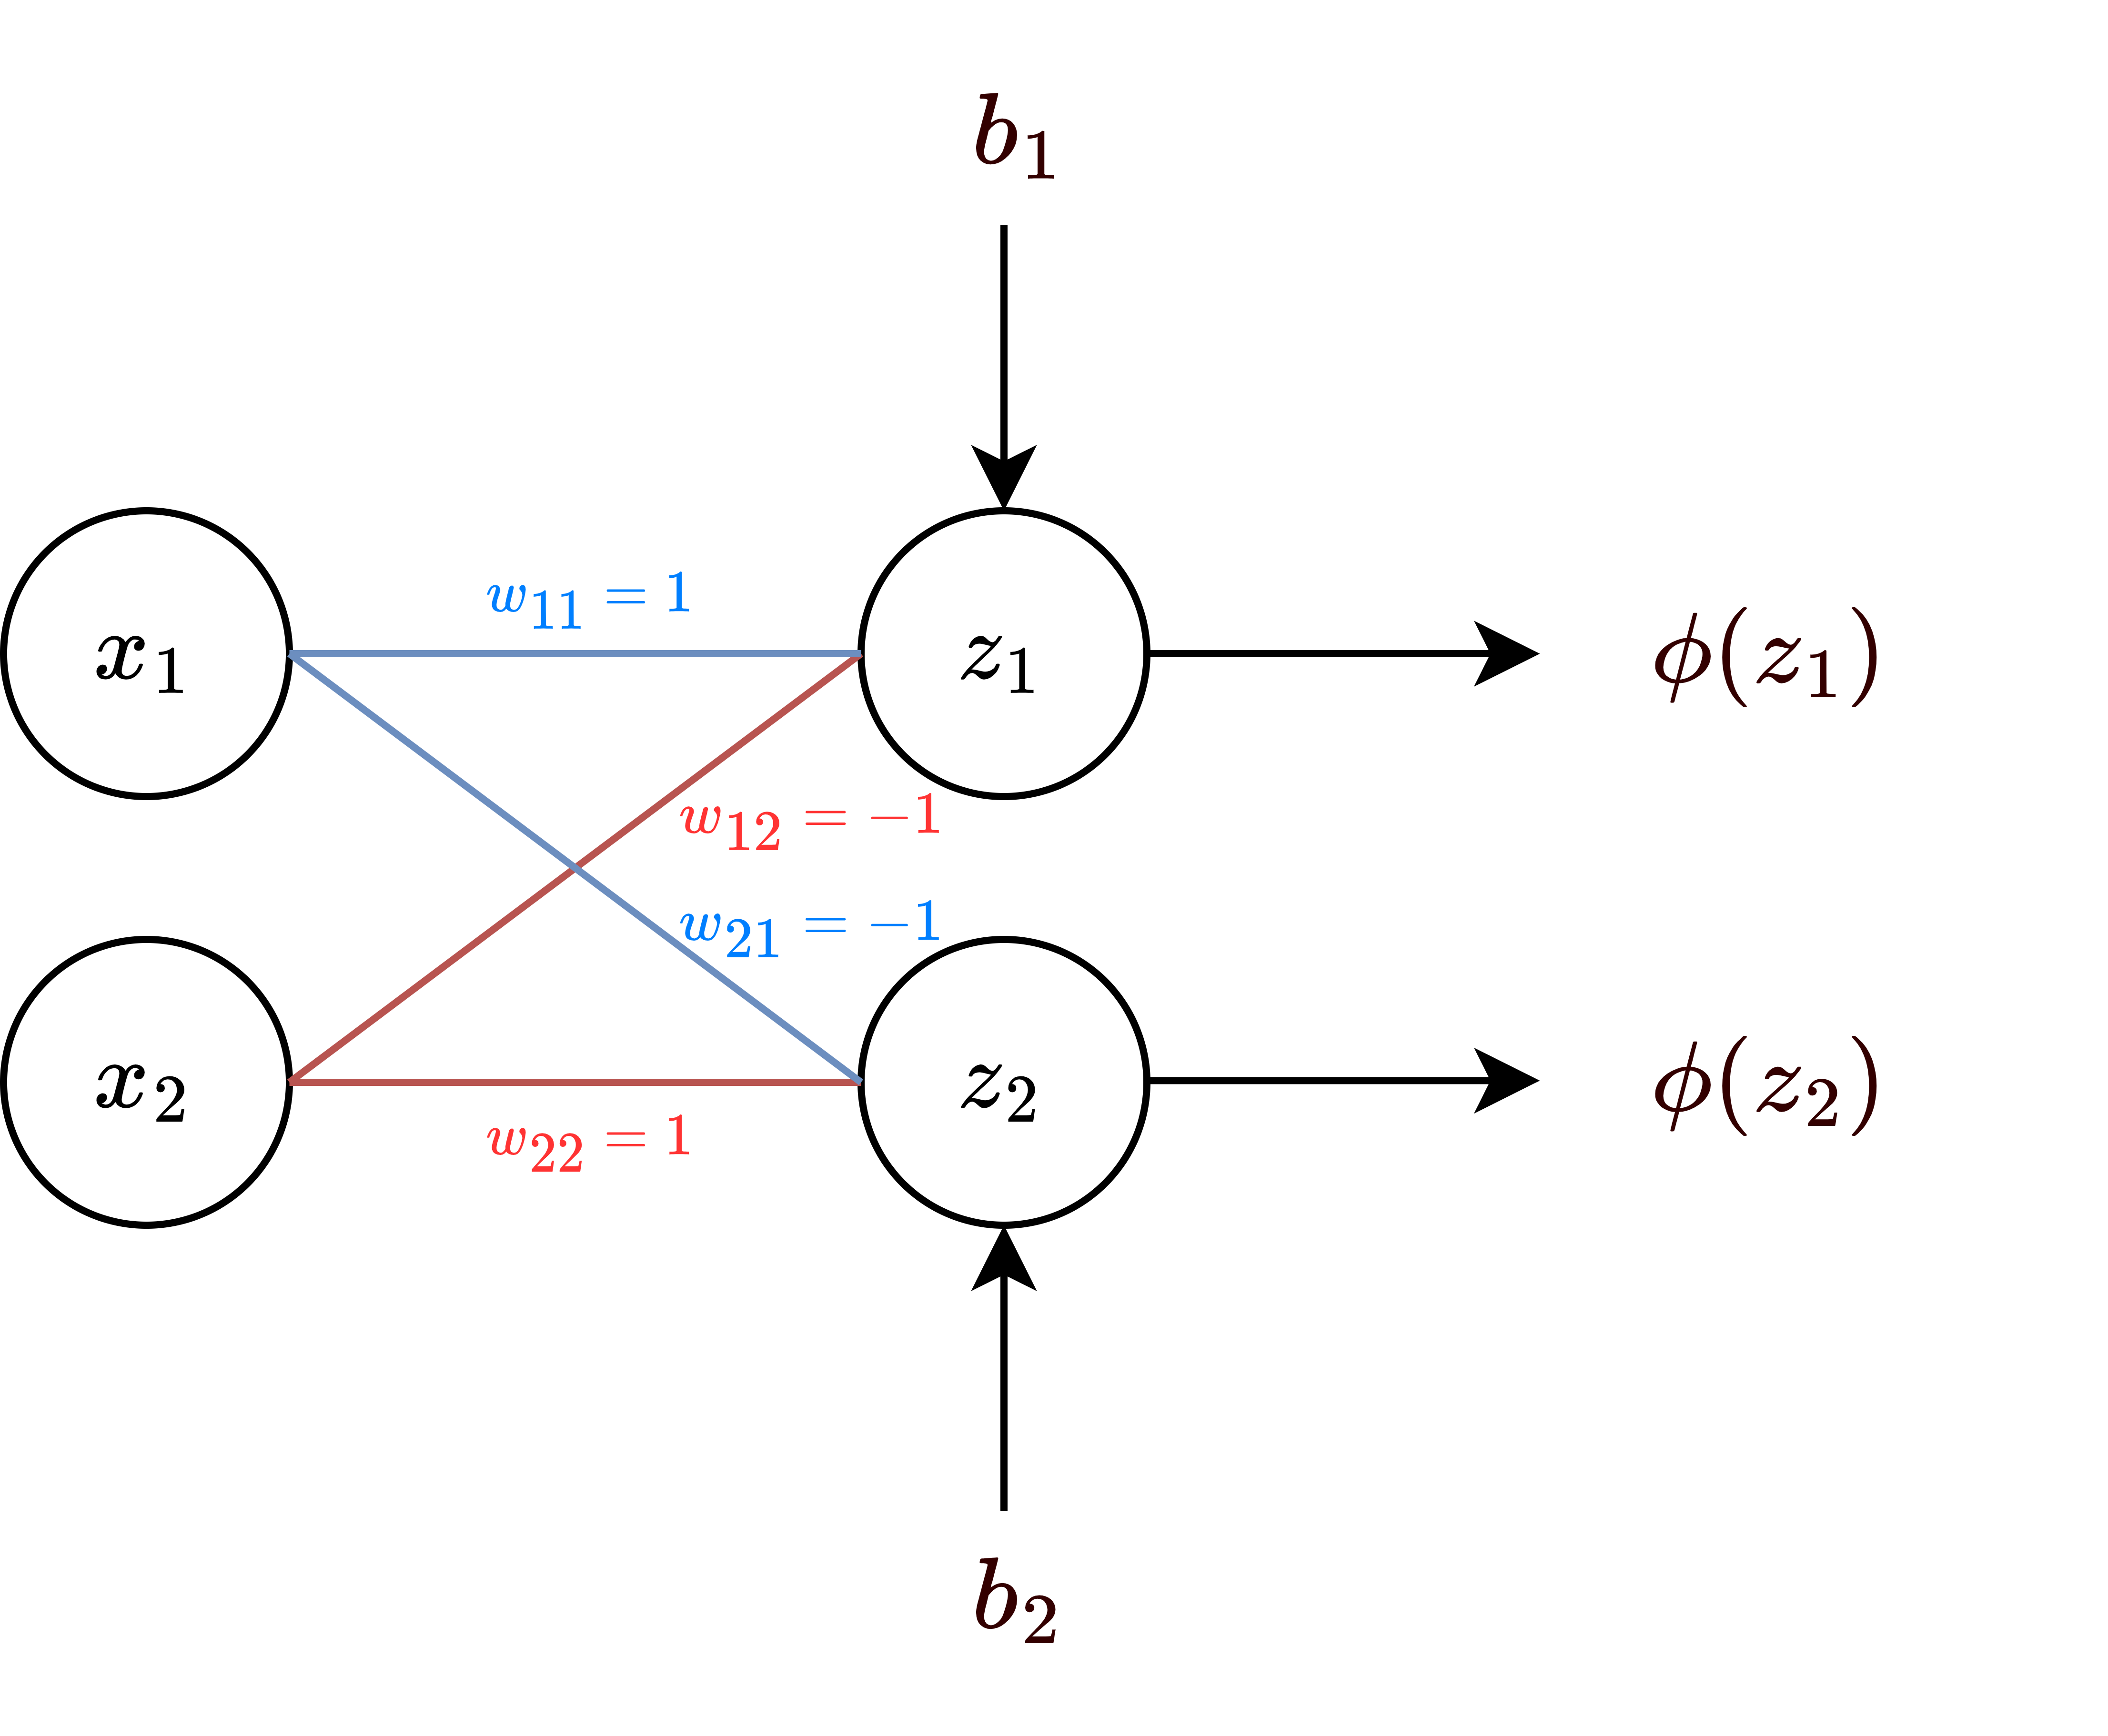
\includegraphics[scale=1.5]{CHAPTER_2/c2_fig_hidden_layer_draw.png}
  \caption{FFN hidden layer}
  \label{fig:hidden_layer_only}
\end{figure} \\
Thus we obtain the system below for the hidden layer.
\begin{align}
  \begin{bmatrix}
    z_1 \\
    z_2
  \end{bmatrix} = \begin{bmatrix}
    b_1 & w_{11} & w_{12}   \\
    b_1 & w_{21} & w_{22}
  \end{bmatrix} \begin{bmatrix}
    1\\
    x_1 \\
    x_2
  \end{bmatrix}
\end{align}
We then feed forward the information from the hidden layer to another layer.
\begin{align}
  \begin{bmatrix}
    h_1 \\
    h_2
  \end{bmatrix} = \phi\begin{pmatrix}
    \begin{bmatrix}
      z_1 \\
      z_2
    \end{bmatrix}
  \end{pmatrix}
\end{align}
At the hidden layer, we are left with the following truth table.
\begin{table}[H]
  \begin{center}
    \begin{tabular}{ c c c c}
      $x_1$ & $x_2$ & XOR \\
     \hline 
      0 & 0 & 0 & \\  
      1 & 0 & 1 & \\  
      0 & 0 & 0 & \text{redundant}\\  
      0 & 1 & 1 & 
    \end{tabular}
    \caption{Truth Table from hidden layer}
  \label{table:truth_table_hidden_layer}
  \end{center}  
\end{table}
\noindent The XOR problem can not be separated from using another perceptron after the hidden layer.
\begin{figure}[H]
  \centering
  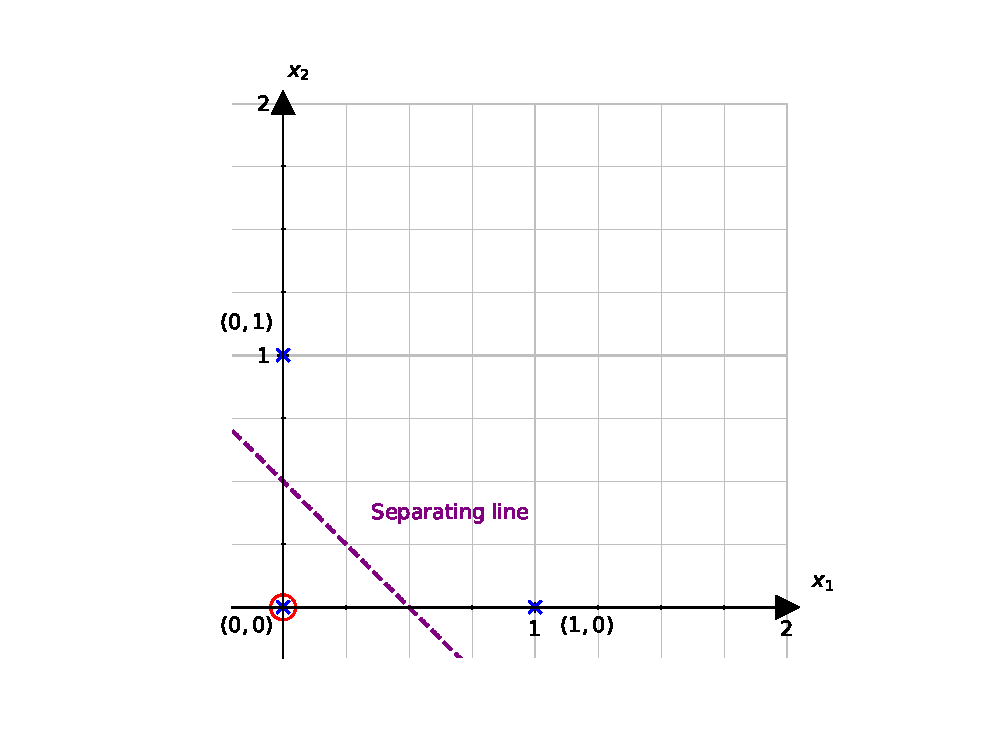
\includegraphics[scale=0.75]{CHAPTER_2/c2_fig_XOR_sep_python.eps}
  \caption{Representation of the hidden layer}
  \label{fig:XOR layer}
\end{figure}
\noindent The equation of the separation line is in figure (\ref{fig:XOR layer}) is given binary
\begin{align}
h_1 + h_2 - \dfrac{1}{2} = 0  
\end{align}
We can now transform the separating line in the form of $\textbf{w}^T\textbf{x} = 0$ to fit the perceptron.
\begin{align}
  \begin{matrix}
    \textbf{w} = \begin{bmatrix}
      -0.5 \\
      1 \\
      1
    \end{bmatrix} & \textbf{h} = \begin{bmatrix}
      1 \\
      h_1 \\
      h_2
    \end{bmatrix}  
  \end{matrix}
\end{align}
Finally, the XOR function can be represented using the set of transform defined below.
\begin{align}
  \begin{matrix}
    f(x_1,x_2) = \phi^{'} \begin{pmatrix}
    \textbf{w}_2^T 
    \begin{pmatrix}
      \phi \begin{pmatrix}
        \textbf{w}_1^T\textbf{x}
    \end{pmatrix}  
  \end{pmatrix}
  \end{pmatrix}
\end{matrix}
\end{align}
where
\begin{align}
  \begin{matrix}
  \textbf{x} = \begin{bmatrix}
    1 \\
    x_1 \\
    x_2
  \end{bmatrix} & \textbf{w}_1 = \begin{bmatrix}
    -0.5 & -0.5 \\
    1 & -1  \\
    -1 & 1 
  \end{bmatrix} & \textbf{w}_2 = \begin{bmatrix}
    -0.5 \\
    1 \\
    1
  \end{bmatrix} 
  \end{matrix}
\end{align}
$\phi^{*}$ takes an augmented input from the calculation of $\phi(\textbf{w}_1^T \textbf{x})$ to accommodate for the bias.
\begin{figure}[H]
  \centering
  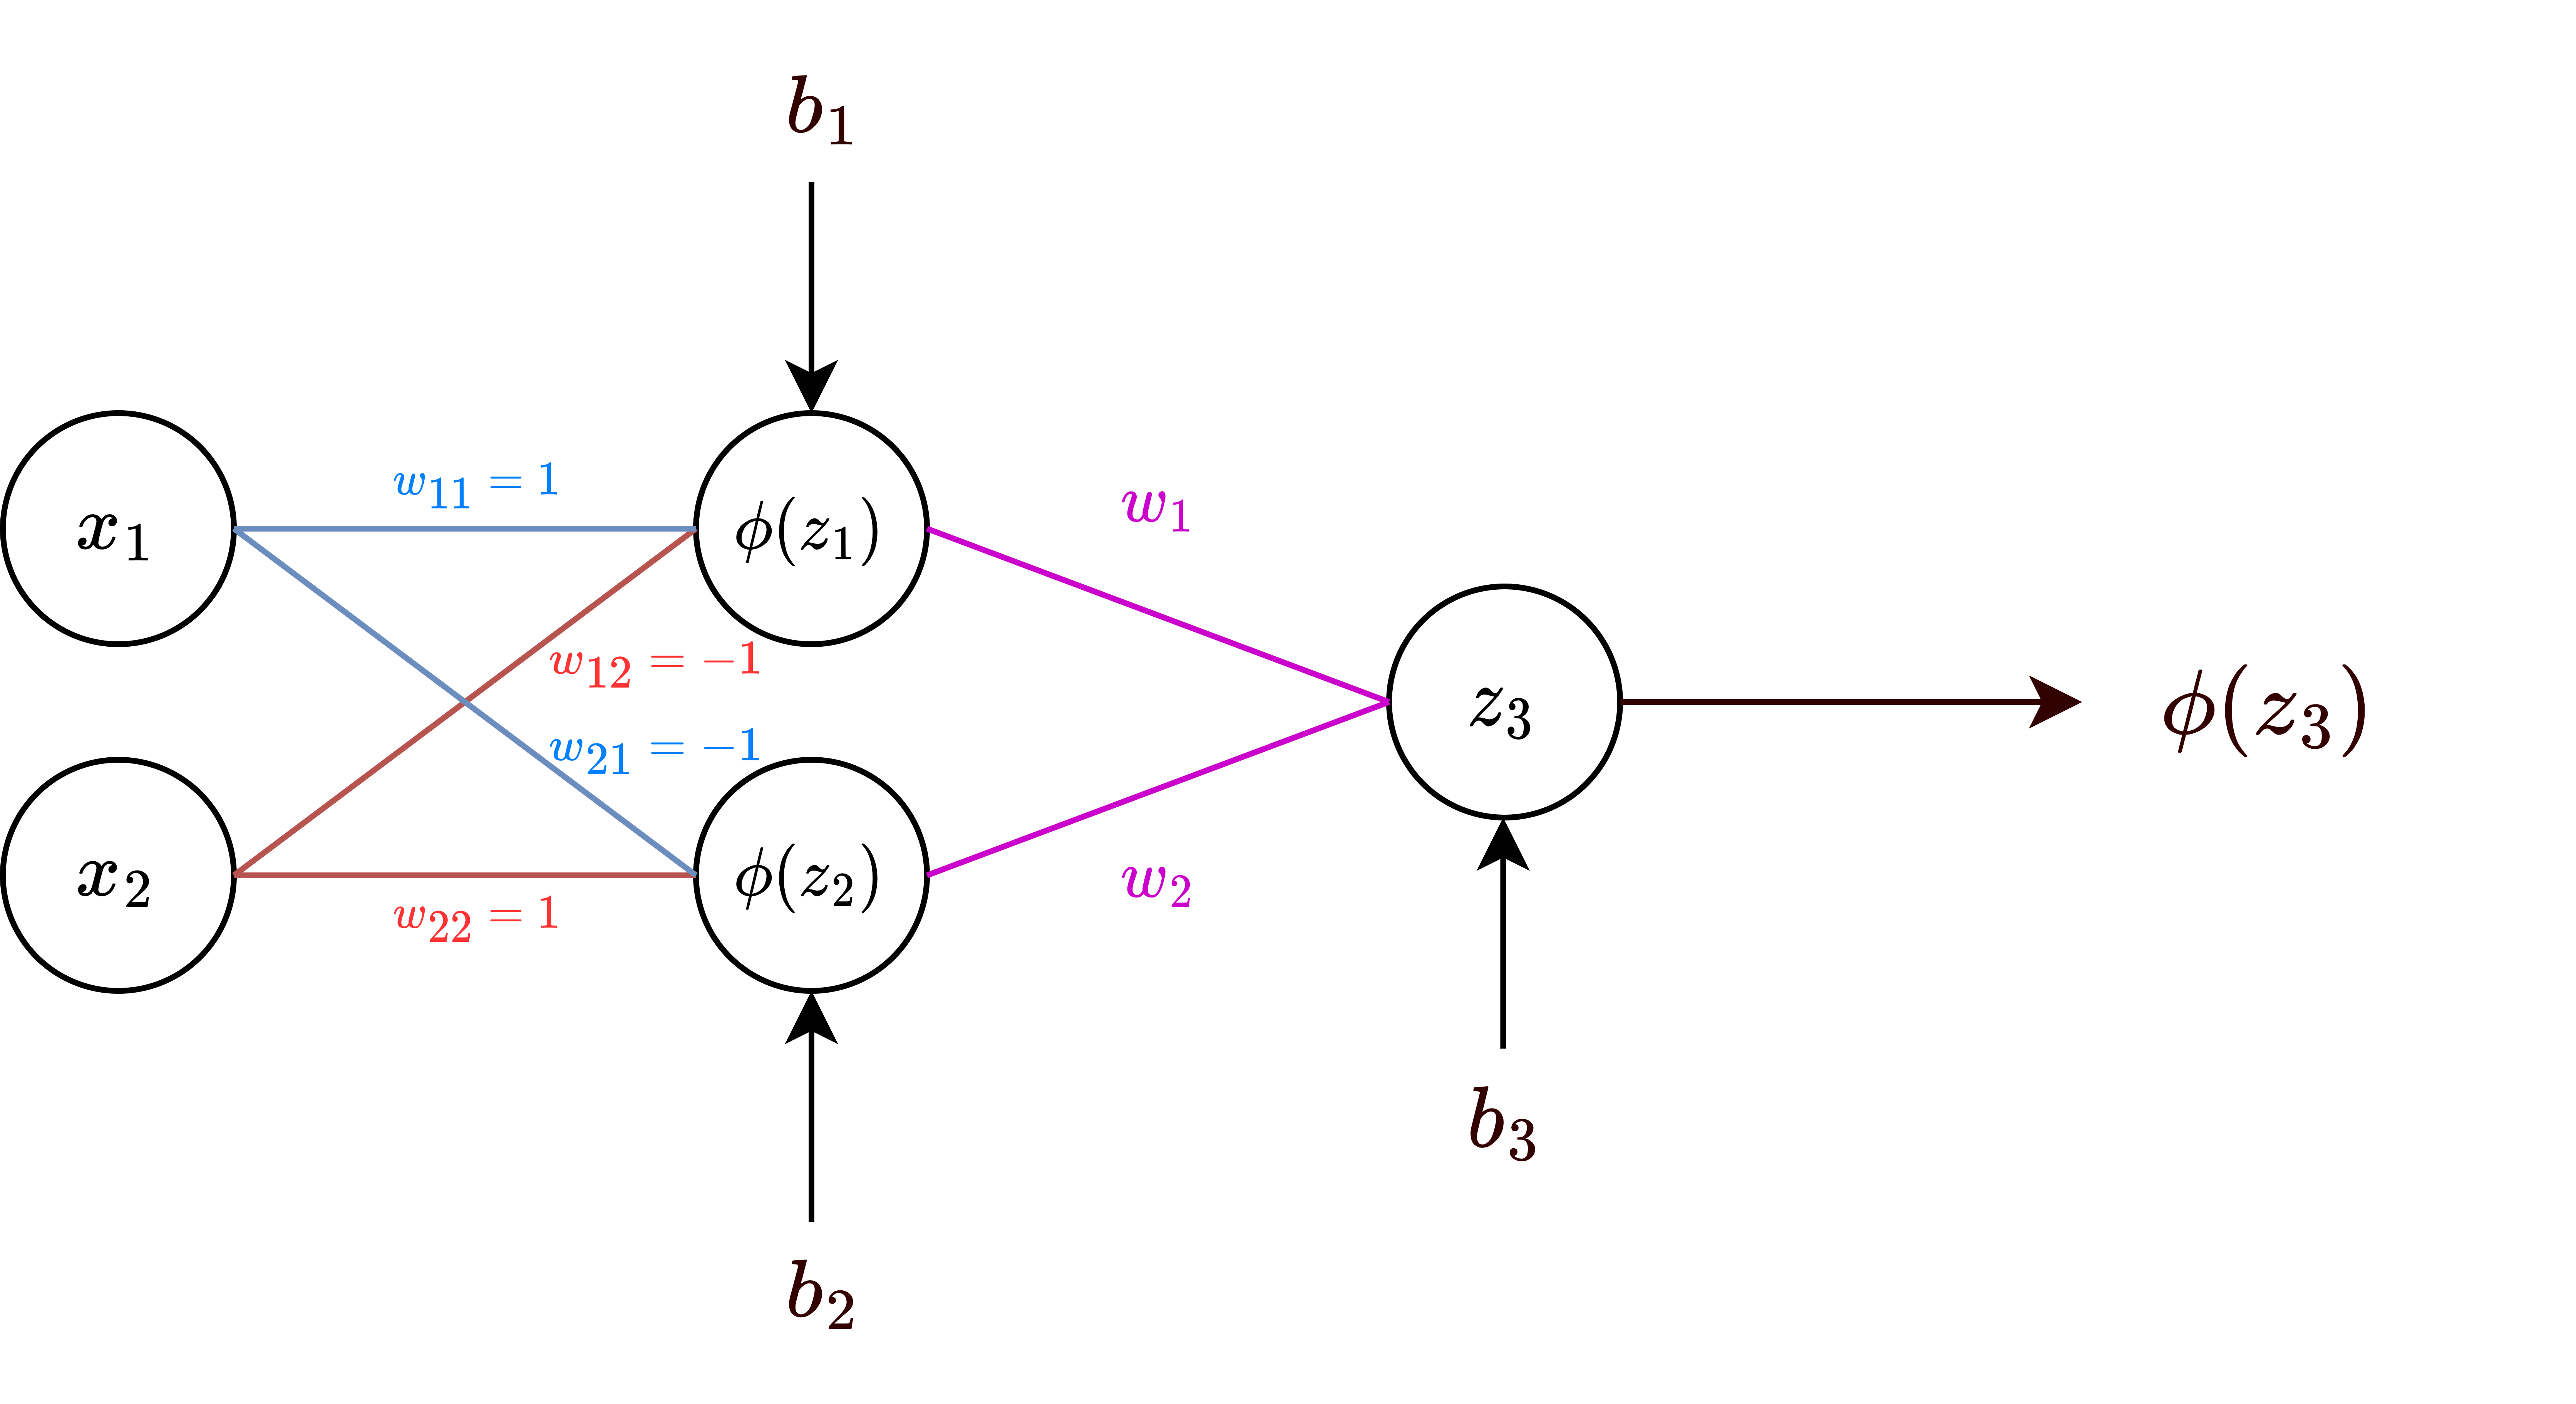
\includegraphics[scale=1.25]{CHAPTER_2/c2_fig_XOR_final_draw.png}
  \caption{Feedforward network for XOR problem}
  \label{fig: ffn_XOR_final}
\end{figure}
\noindent \textbf{Checking for $\textbf{x} = \begin{bmatrix} 1 & 0 & 0 \end{bmatrix}^T$}
\begin{align*}
  \textbf{w}_1^T\textbf{x} &= \begin{bmatrix}
    -0.5 & 1 & -1 \\
    -0.5 & -1 & 1 
  \end{bmatrix} \begin{bmatrix}
    1\\
    0 \\
    0
  \end{bmatrix} = \begin{bmatrix}
    -0.5 \\
    -0.5
  \end{bmatrix} \\
  \phi(\textbf{w}_1^T\textbf{x}) &= \phi\begin{pmatrix}
    \begin{bmatrix}
      -0.5 \\
      -0.5
    \end{bmatrix}
  \end{pmatrix} = \begin{bmatrix}
    0 \\
    0
  \end{bmatrix} \\
  \phi^{*} \begin{pmatrix}
    \textbf{w}_2^T 
    \begin{pmatrix}
      \phi \begin{pmatrix}
        \textbf{w}_1^T\textbf{x}
    \end{pmatrix}  
  \end{pmatrix}
  \end{pmatrix} &= \phi^{*}\begin{pmatrix}
    \begin{bmatrix}
      -0.5 & 1 & 1
    \end{bmatrix} \begin{bmatrix}
      1 \\ 
      0 \\
      0
    \end{bmatrix}
  \end{pmatrix} = \phi^{*}(-0.5)
\end{align*}
Thus, for $\textbf{p}_1 = \begin{bmatrix}
  0,0
\end{bmatrix}^T$
\begin{align*}
  f(x_1,x_2) = \phi^{*} (-0.5) = 0
\end{align*}
\textbf{Checking for $\textbf{x} = \begin{bmatrix} 1 & 0 & 1 \end{bmatrix}^T$}
\begin{align*}
  \textbf{w}_1^T\textbf{x} &= \begin{bmatrix}
    -0.5 & 1 & -1 \\
    -0.5 & -1 & 1 
  \end{bmatrix} \begin{bmatrix}
    1\\
    0 \\
    1
  \end{bmatrix} = \begin{bmatrix}
    -1.5 \\
    0.5
  \end{bmatrix} \\
  \phi(\textbf{w}_1^T\textbf{x}) &= \phi\begin{pmatrix}
    \begin{bmatrix}
      -1.5 \\
      0.5
    \end{bmatrix}
  \end{pmatrix} = \begin{bmatrix}
    0 \\
    1
  \end{bmatrix} \\
  \phi^{*} \begin{pmatrix}
    \textbf{w}_2^T 
    \begin{pmatrix}
      \phi \begin{pmatrix}
        \textbf{w}_1^T\textbf{x}
    \end{pmatrix}  
  \end{pmatrix}
  \end{pmatrix} &= \phi^{*}\begin{pmatrix}
    \begin{bmatrix}
      -0.5 & 1 & 1
    \end{bmatrix} \begin{bmatrix}
      1 \\ 
      0 \\
      1
    \end{bmatrix}
  \end{pmatrix} = \phi^{*}(0.5)
\end{align*}
Thus, for $\textbf{p}_4 = \begin{bmatrix}
  0,0
\end{bmatrix}^T$
\begin{align*}
  f(x_1,x_2) = \phi^{*} (0.5) = 1
\end{align*}
\section{Activation Function}
The hard-delimiters used in our previous feedforward network are linear. However, different activation functions can use with a perceptron to introduce non-linearity in our network. The non-linearity enables a wider range of problems to be tackled. The function to be used is subjective to the problem being solved and the form of the desired result we want. Some common activation functions are defined below.
\begin{align}
\intertext{Linear}
  \phi(z) = z
\end{align}
\begin{align}
\intertext{Unit Step (Heaviside Function)}
  \phi(z) = \begin{cases}
    0 & z<0 \\
    0.5 & z=0 \\
    1 & z>0
  \end{cases}
\end{align}
\begin{align}
  \intertext{Signum}
  \phi(z) = \begin{cases}
    -1 & z<0 \\
    0 & z=0 \\
    1 & z>0
  \end{cases}
\end{align}
\begin{align}
  \intertext{Sigmoid}
  \phi(z) = \frac{1}{1+ e^{-z}}
\end{align}
\begin{align}
  \intertext{Hyperbolic Tangent(tanh)}
  \phi(z) = \frac{e^z - e^{-z}}{e^z + e^{-z}}
\end{align}
\begin{align}
  \intertext{ReLU}
  \phi(z) = \begin{cases}
    0 & z<0 \\
    z & z>0
  \end{cases}
\end{align}
\newpage
\section{Backpropagation}
We have seen how information flows in a feedforward neural network. Backpropagation algorithm is the process of spreading the error at the output layer throughout the other layers in the network. The goal is to understand how does the error changes with respect to the weights and biases. Consider the neural network below with $N$ number of layers (including the input and output layer).\vspace{10mm}
\begin{figure}[H]
  \centering
  \includegraphics[scale=1.15]{CHAPTER_2/c2_bp_nn_draw.png}
  \vspace{10mm}
  \caption{Neural Network with $N$ number of layers}
  \label{fig:bp_nn_complete}
\end{figure}\vspace{10mm}
\noindent The annotation between two consecutive layers, $l$ and $l+1$, in the network is given by the following set of indexed values.
\begin{center}
  \begin{tabular}{p{0.06\linewidth} p{0.03\linewidth} p{0.82\linewidth}}
    $b_j^{l+1}$ & $\rightarrow$ & Bias input at the $j^{th}$ neuron in the ${l+1}^{th}$ layer \\ 
    $w_{jk}^{l+1}$ & $\rightarrow$ & Weight between the $k^{th}$ and $j^{th}$ neuron in the $l^{th}$ and ${(l+1)}^{th}$ layer respectively \\  
    $z_j^{l+1}$ &$\rightarrow$& Input of the activation function at the $j^{th}$ neuron in the $(l+1)^{th}$ layer \\
    $a_j^l$ & $\rightarrow$ & Output from the activation function at the $j^{th}$ neuron in the $l^{th}$ layer
  \end{tabular}
\end{center}
\begin{figure}[ht]
  \centering
  \includegraphics[scale=1.05]{CHAPTER_2/c2_bb_nn_cons_draw.png}
  \caption{Consecutive layers, $l$ and $l+1$, in a neural network}
  \label{fig:bp_nn_complete_cons_layer}
\end{figure}
Let the activation function be denoted as $\sigma$ such that
\begin{align}
  \label{eq:activation_function_at_l+1 layer}
  a_j^{(l+1)} &= \sigma\begin{pmatrix}
    z_j^{(l+1)}
  \end{pmatrix} \\
  \label{eq:input of activation_function_at_l+1 layer}
  z_j^{(l+1)} &= \sum_kw_{jk}^{(l+1)}a_k^{(l)} + b_j^{(l+1)}
\end{align}
We start at the end of the network by calculating the value of the cost/error function. Let $C$ be the cost function which takes as input the output layer
\begin{align}
  \label{eq:cost_function_definition}
  C &= C\begin{pmatrix}
    a_j^L
  \end{pmatrix} \\
    &=\dfrac{1}{2} \sum_j (y_j - a_j^{L})^2  
    \nonumber
\end{align}
where $y_j$ is the desired exact value that we want the network to predict. Also, let the change in the cost function with respect to the input of the activation function be given by $\delta_j^L$ where 
\begin{align*}
  \delta_j^L &= \dfrac{\partial C}{\partial z_j^L}
\intertext{Using result (\refeq{eq:activation_function_at_l+1 layer}) and the definition (\refeq{eq:cost_function_definition})}
  \delta_j^L &= \dfrac{\partial C(a_j^L)}{\partial z_j^L} \\
  &= \dfrac{\partial C(\sigma(z_j^L))}{\partial z_j^L}
\intertext{Applying the chain rule}
  \delta_j^L &= \dfrac{\partial C(\sigma(z_j^L))}{\partial z_j^L} \\
  &= \dfrac{\partial C }{\partial a_j^L}  \dfrac{\partial a_j^L}{\partial z_j^L}
\end{align*}
From equation (\refeq{eq:activation_function_at_l+1 layer})
\begin{align*}
  a_j^{(L)} &= \sigma(
    z_j^{(L)} ) \\
  \dfrac{\partial a_j^{(L)}}{\partial z_j^{(L)}} &= \sigma^{'}(
    z_j^{(L)})
\end{align*}
Thus, the change in the cost function with respect to the input of the activation function in the last layer is given by 
\begin{align}
  \label{eq:BP_EQ_VEC_1}
  \delta_j^{(L)} = \dfrac{\partial C }{\partial a_j^{(L)}} \sigma^{'}(z_j^{(L)})
\end{align}
Next, we find how to back-propagate the changes from an upper layer $l+1$ to the previous layer $l$. Consider the change in the cost function based at the $l^{th}$ layer 
\begin{align}
  \label{eq: change_at_layer_l}
  \delta_j^{(l)} = \dfrac{\partial C}{\partial z_j^{(l)}}
\end{align}
From figure (\ref{fig:bp_nn_complete_cons_layer}); an element in the $l^{th}$ layer influences all the neurons in the $(l+1)^{th}$ layer. Thus, when applying the chain rule we sum over all the neurons which gives
\begin{align}
  \label{eq: delta_of_cost_bet_layers}
  \delta_j^l &= \sum_k \frac{\partial C}{\partial z_k^{(l+1)}} \dfrac{\partial z_k^{(l+1)}}{\partial z_j^{(l)}}
\intertext{From equations (\refeq{eq:activation_function_at_l+1 layer}) and (\refeq{eq:input of activation_function_at_l+1 layer})}
\nonumber
\dfrac{\partial z_k^{(l+1)}}{\partial z_j^{(l)}} &= \dfrac{\partial}{\partial z_j^{(l)}} \Big(\sum_sw_{ks}^{(l+1)}\sigma(z_s^{(l)}) + b_k^{(l+1)}\Big) \\
\nonumber
&=\sum_sw_{ks}^{(l+1)}\dfrac{\partial \sigma(z_s^{(l)})}{\partial z_j^{(l)}} \\
\nonumber
&= \sum_sw_{ks}^{(l+1)}\sigma^{'}(z_s^{(l)}) \dfrac{\partial z_s^{(l)}}{\partial z_j^{(l)}} \\
\intertext{The partial derivative only exist and is 1 when $s=j$; else the value is 0.}
\label{eq: z_j partials}
\dfrac{\partial z_k^{(l+1)}}{\partial z_j^{(l)}}  &= w_{kj}^{(l+1)} \sigma^{'}(z_j^{(l)})
\end{align}
Substituting (\refeq{eq: z_j partials}) and (\refeq{eq: change_at_layer_l}) into (\refeq{eq: delta_of_cost_bet_layers})
\begin{align}
  \label{eq:BP_EQ_VEC_2}
  \delta_j^l = \sum_k \delta_k^{(l+1)} w_{kj}^{(l+1)} \sigma^{'}(z_j^{(l)})
\end{align}
Equation (\ref{eq:BP_EQ_VEC_2}) are the changes in $l^{th}$ layer from the changes that happened in the $(l+1)^{th}$ layer. Since we do not explicitly adjust the output and input of the activation functions, we derive the changes of the cost function with respect to the bias and weight. Consider the effect of the bias at each layer given by 
\begin{align*}
  \dfrac{\partial C}{\partial b_j^{(l)}} &= \dfrac{\partial C}{\partial z_j^{(l)}} \dfrac{\partial z_j^{(l)}}{\partial b_j^{(l)}} \\
\end{align*}
Using equation (\refeq{eq:input of activation_function_at_l+1 layer})
\begin{align*}
  \dfrac{\partial z_j^{(l)}}{\partial b_j^{(l)}} &= \dfrac{\partial}{\partial b_j^{(l)}} \Big(  \sum_kw_{jk}^{(l+1)}a_k^{(l)} + b_j^{(l+1)}  \Big) \\
  &= 1
\end{align*}
Thus, the change of in the cost function with respect to the bias at any layer is given by 
\begin{align}
  \label{eq:BP_EQ_VEC_3}
  \dfrac{\partial C}{\partial b_j^{(l)}} = \delta_i^{(j)}
\end{align}
Finally, consider the rate of change of the cost function with respect to any weight in the network given by 
\begin{align}
  \label{eq: partial_C_with_weight}
  \dfrac{\partial C}{\partial w_{jk}^{(l)}} = \dfrac{\partial C}{\partial z_m^{(l)}} \dfrac{\partial z_m^{(l)}}{\partial w_{jk}^{(l)}}
\end{align}
Using equation (\refeq{eq:input of activation_function_at_l+1 layer})
\begin{align}
  \nonumber
  \dfrac{\partial z_m^{(l)}}{\partial w_{jk}^{(l)}} &= \dfrac{\partial}{\partial w_{jk}^{(l)}} \Big(  \sum_sw_{ms}^{(l)}a_s^{(l-1)} + b_m^{(l)}  \Big) \\
  \nonumber
  &= \sum_s a_s^{(l-1)} \dfrac{\partial w_{ms}^{(l)}}{\partial w_{jk}^{(l)}}
\end{align}
The partial derivative only exist and is 1 when $s=k$ and $m=j$; else the value is 0.
\begin{align}
  \label{eq: partial_act_weight}
  \dfrac{\partial z_j^{(l)}}{\partial w_{jk}^{(l)}} &= a_k^{(l-1)}
\end{align}
Substituting (\refeq{eq: z_j partials}) and (\refeq{eq: partial_act_weight}) into (\refeq{eq: partial_C_with_weight})
\begin{align}
  \label{eq:BP_EQ_VEC_4}
  \dfrac{\partial C}{\partial w_{jk}^{(l)}} = \delta_j^{(l)}a_k^{(l-1)}
\end{align}
The four main back-propagation equations are given by 
\begin{align}
  \delta_j^{(L)} &= \dfrac{\partial C }{\partial a_j^{(L)}} \sigma^{'}(z_j^{(L)}) \\
  \delta_j^l &= \sum_k \delta_k^{(l+1)} w_{kj}^{(l+1)} \sigma^{'}(z_j^{(l)})\\
  \dfrac{\partial C}{\partial b_j^{(l)}} &= \delta_i^{(j)} \\
  \dfrac{\partial C}{\partial w_{jk}^{(l)}} &= \delta_j^{(l)}a_k^{(l-1)}
\end{align}
We vectorize the above set of equations by using the Hadamard product. Given two matrices of the $A$ and $B$ of the same dimension, $m \times n$, the Hadamard product is given as
\begin{align*}
  (A \odot B)_{mn} = (A)_{mn} (B)_{mn} 
\end{align*}
The vectorized form of the back-propagation equations are given by 
\begin{align}
  \delta^{(L)} &= \nabla_{a^{(L)}}C \odot \sigma^{'}(z^{(L)}) \\
  \delta^{(l)} &= (w^{(l+1)})^T\sigma^{(l+1)} \odot \sigma^{'}(z^{(l)}) \\
  \nabla_{b^{(l)}} C &= \delta^{(l)} \\
  \nabla_{w^{(l)}} C &= \delta^{(l)}a^{(l-1)}
\end{align}
\begin{algorithm}[H]
  \caption{Back-Propagation Algorithm}\label{alg:back_propagation_algo}
  \begin{algorithmic}[1]
  \State{\textbf{Start}}
  \State{\textbf{Step 1} (Input)}
  Compute the first activation layer $a^{(1)}$ using input values $x$ \\
  \, \, \, $a^{(1)} = \sigma(w^{(1)}x + b^{(1)} )$
  \State {\textbf{Step 2} (Feed-Forward)}\\
  \, \, \, Feed forward the input to the next layers
  \For{$l = 2,3,\dots,L$}
    \State{$z^{(l)} = w^{(l)}a^{(l-1)}+b^{(l)}$}
    \State $a^{(l)} = \sigma(z^{(l)})$
  \EndFor  
  \State \textbf{Step 3} (Cost/Error Calculation)\\
  \, \, \, Compute the cost function, $C$, at the output layer $L$
  \State \textbf{Step 4} (Backpropagate) \\
  \, \, \, Compute the rate of change of the cost function $w.r.t$ to $z^{(L)}$\\
  \, \, \,  $\delta^{(L)} = \nabla_{a^{(L)}}C \odot \sigma^{'}(z^{(L)})$
  \For{$l = L-1, L-2, \dots, 2$}
    \State $\delta^{(l)} = (w^{(l+1)})^T\sigma^{(l+1)} \odot \sigma^{'}(z^{(l)})$
    \State $\nabla_{b^{(l)}} C = \delta^{(l)}$
    \State $\nabla_{w^{(l)}} C = \delta^{(l)}a^{(l-1)}$
  \EndFor
\end{algorithmic}
\end{algorithm}
\section{Sequential Neural Networks}
\subsubsection*{Recurrent Neural Network(RNN)}
Developed through the work of \cite{Rumelhart:1986aa}, a recurrent neural network is a type of neural network capable of modelling sequential data for predictions. Like to the feedforward network, the RNN consists of an input layer and  an output layer with a hidden state instead of a hidden layer. The hidden state act as a feedback loop. That is, the output at a particular step in the sequence is fed to the next step's input to compute the next step's output. Hence, recurrent neural networks are neural networks with hidden states. Consider the sequential input data $\mathbf{X}_t \in \mathbb{R}^{n \times d}$, with batch size $n$ and $d$ inputs, at a particular time step $t$, $\mathbf{H}_t \in \mathbb{R}^{n \times h}$ be the hidden layer, $\mathbf{W}_{xh}\in \mathbb{R}^{d \times h}$  be the weight applied on the input data, $\mathbf{W}_{hh}\in \mathbb{R}^{h \times h}$ be the weight applied to the output hidden state, $\mathbf{b}_h \in \mathbb{R}^{1 \times h}$ and $\phi$ be the activation function; thus the calculation at the hidden layer is given by:
\begin{align}
  \label{eq:RNN_HL}
  \mathbf{H}_t = \phi(\mathbf{X}_t \mathbf{W}_{xh} + \mathbf{H}_{t-1}\mathbf{W}_{hh} + \mathbf{b}_h)
\end{align}
Consider the weights $\mathbf{W}_{hq} \in \mathbb{R}^{d \times h}$ and the bias $\mathbf{b}_h \in \mathbb{R}^{1 \times q}$, thus the computation at the output layer is given by:
\begin{align}
  \label{eq:RNN_OL}
  \mathbf{O}_t = \mathbf{H}_t \mathbf{W}_{hq} + \mathbf{b}_q
\end{align}
\begin{figure}[H]
  \centering
  \includegraphics[scale=0.8]{CHAPTER_2/c2_fig_RNN_draw.png}
  \caption{An RNN with a hidden state}
  \label{}
\end{figure}
\noindent As we unfold a recurrent neural network for more time steps, the number of parameters does not increase. The input of the activation function gets recursively very large or very small. Consequently, we are limited by the problem of vanishing or exploding gradients when optimizing recurrent neural networks \cite{Bengio1994} \cite{Kolen2001}. A preventive measure would be to truncate the recursive gradient term during backpropagation. RNNs also suffer from short-term memory; important information in very long sequence from the beginning are left out.
\subsubsection*{Long Short Term Memory(LSTM)}
Introduced in 1997 by \cite{Hochreiter1997}, the long short-term memory model was introduced to solve the vanishing and exploding problem in the RNN. While the architecture is similar to the RNN, the LSTM replaces the hidden state with a memory cell. The memory cell comprises three main “gates” and an input node: the forget gate, the input gate, the output gate  and the input node, respectively. The forget gate controls whether or not we keep the input from the previous hidden state.  The input gate determines how much of the input should contribute to the internal cell memory and be passed to the input node. The memory cell is calculated at the input node using the input value and the value from the input gate. Finally, the output gate determines how much of the memory cell of the current time step impacts the next time step in the next memory cell. Consider the input $\mathbf{X}_t \in \mathbb{R}^{n \times d}$, the hidden state of the previous time step be  $\mathbf{H}_t \in \mathbb{R}^{n \times h}$, the input gate be given by $\mathbf{I}_t \in \mathbb{R}^{n \times h}$, the forget gate given by $\mathbf{F}_t \in \mathbb{R}^{n \times h}$, the input node given by $\tilde{\mathbf{C}_t} \in \mathbb{R}^{n \times h}$,  the output gate be $\mathbf{O}_t \in \mathbb{R}^{n \times h}$ and the memory cell state be given by $\mathbf{C}_t \in \mathbb{R}^{n \times h}$ then the computations of the LSTM are given by:
\begin{align}
  \label{eq:LSTM_HS}
  \mathbf{I}_t &= \sigma(\mathbf{X}_t \mathbf{W}_{xi} + \mathbf{H}_{t-1}\mathbf{W}_{hi} + \mathbf{b}_i) \\
  \mathbf{F}_t &= \sigma(\mathbf{X}_t \mathbf{W}_{xf} + \mathbf{H}_{t-1}\mathbf{W}_{hf} + \mathbf{b}_f) \\
  \mathbf{O}_t &= \sigma(\mathbf{X}_t \mathbf{W}_{xo} + \mathbf{H}_{t-1}\mathbf{W}_{ho} + \mathbf{b}_o) \\
  \tilde{\mathbf{C}_t} &= \tanh(\mathbf{X}_t \mathbf{W}_{xc} + \mathbf{H}_{t-1}\mathbf{W}_{hc} + \mathbf{b}_c)\\
  \mathbf{C}_t &= \mathbf{F}_t \odot \mathbf{C}_{t-1} + \mathbf{I}_t \odot \tilde{\mathbf{C}_t}
\end{align}
where $ \mathbf{W}_{xi}$, $ \mathbf{W}_{xf}$, $ \mathbf{W}_{xo}$,  $\mathbf{W}_{xc}$ $\in \mathbb{R}^{d \times h}$ and $ \mathbf{W}_{hi}$, $ \mathbf{W}_{hf}$, $ \mathbf{W}_{ho}$,  $\mathbf{W}_{hc}$ $\in \mathbb{R}^{h \times h}$ are weight parameters and $\mathbf{b}_i$, $\mathbf{b}_f$, $\mathbf{b}_o$, $\mathbf{b}_c$ $\in \mathbb{R}^{1 \times h}$ are the bias parameters.
\begin{figure}[H]
  \centering
  \includegraphics[scale=0.76]{CHAPTER_2/c2_fig_LSTM_draw.png}
  \caption{Computing the hidden state in an LSTM model}
  \label{LSTM_LAYER}
\end{figure}
\noindent LSTM addresses the vanishing and exploding gradient problem of the RNN by controlling the amount of information being carried to the memory and providing a continuous gradient flow to facilitate backpropagation. Many variants of LSTM have been developed over the years due to their dominance in sequence learning. Some LTSM variants are: The Peephole Variant, the Coupled Gate Variation, Gated Recurrent Units (GRU). However, they are pretty costly to compute due to their long-range dependencies on the sequence.
\subsubsection*{Bidirectional RNN(BRNN)}
In order to overcome the uni-direction learning of RNN and LSTM,\cite{Schurster1997} introduced the bidirectional recurrent neural network. The implementation consists of two unidirectional layers chained together in opposite directions but taking the same inputs. The output is obtained by concatenating the two directional outputs from the hidden layers. The obtained layers is then computed to get the prediction. Consider the input $X_t \in \mathbf{R}^n$ for time step $t$, the forward and backward hidden unidirectional layers for time step $t$ be given by $\overrightarrow{H_t} \in \mathbb{R}^{n \times h}$ and $\overleftarrow{H_t} \in \mathbb{R}^{n \times h}$ respectively and the output layer be given by $\mathbf{O}_t$, then the computations of the BRNN is given by:
\begin{align}
  \label{eq:BRNN_LAYER}
  \overrightarrow{H_t} &= \phi(\mathbf{X}_{t} \mathbf{W}_{xh}^{(f)} + \overrightarrow{\mathbf{H}}_{t-1}\mathbf{W}_{hh}^{(f)} + \mathbf{b}_h^{(f)}) \\
  \overleftarrow{H_t}&= \phi(\mathbf{X}_t \mathbf{W}_{xh}^{(b)} + \overleftarrow{\mathbf{H}}_{t+1}\mathbf{W}_{hh}^{(b)} + \mathbf{b}_h^{(b)})\\
  \mathbf{O}_t &= \mathbf{H}_t \mathbf{W}_{tq} + \mathbf{b}_q
  \nonumber
  \intertext{where $\mathbf{W}_{xh}^{(f)}$ and $\mathbf{W}_{xh}^{(b)}$ $\in \mathbb{R}^{d \times h}$, $\mathbf{W}_{hh}^{(f)}$ and $\mathbf{W}_{hh}^{(b)}$ $\in \mathbb{R}^{h\times h}$, $\mathbf{W}_{hq}\in\mathbb{R}^{2h \times q}$ are the weight parameters and  $\mathbf{b}_h^{(f)}$ and $\mathbf{b}_h^{(b)}$ $\in \mathbb{R}^{1 \times h}$ and $\mathbf{b_q} \in \mathbb{R}^{1 \times q}$ are the bias parameters.} \nonumber
\end{align}
\begin{figure}[H]
  \centering
  \includegraphics[scale=0.90]{CHAPTER_2/c2_fig_BRNN_draw.png}
  \caption{Architecture of a bidirectional RNN}
  \label{BRNN_LAYER}
\end{figure}
\noindent Bidirectional recurrent neural networks are very efficient in sequential modelling in cases where context is a priority. Natural language processing, speech recognition, handwriting recognition, and part-of-speech tagging; leverages BRNN as context input is required.